\chapter{Annotation Correction and Building Deformable Models without landmarks}

% Building and training deformable models of objects (e.g. faces, ears, bodies, bottles, vehicles etc.) has recently been widely researched for object detection, part localisation, fitting, recognition and tracking using manual annotated data. Shapes and appearances of majority of objects vary significantly from object instance. To illustrate, ears have complicated inner structures (e.g. helix, crus antihelicis, scapha, tragus, lobe etc.) which differs remarkably between ears and highly sensitive to intensity changes. Recently, we have witnessed a great progress in object detection, alignment and recognition.

% To train deformable models with satisfiable generalisation, large amount of careful manual annotation is required. However, landmark annotation is extremely time consuming, work intensive and, most importantly, number of landmarks have to stay consistent for all training data while it is challenging to maintain the consistency or to avoid bias when annotating objects that having reach features. In ears, for example, large amount of landmarks required as the inner structure of ears are complex. To annotate an ear with clear contour, helix and cavum conchae, more than 50 landmarks are required. The inconsistency of ear features enhanced the difficulty of accurate annotation (e.g. Fossa Triangularies and Crus Helicis are optional feature of an ear also their visibility is highly sensitive to pose and illumination variation).
% To illustrate how much time consuming careful ear annotation is, according to our experience, a trained annotator may need an average of (TODO: experiment) minutes per image for the manual annotation of 55 landmarks. This means that the annotation of 1000 images requires a total of about (TODO: experiment). Furthermore, personal issue, prior knowledge and circumstances can heavily bias the annotation accuracy thus second round correction might desired.

% We propose a framework to (1) construct SDMs using training data with inconsistent annotation, (2) introduce highly effective curve annotation which tremendously reduces manual work overload but maintains same performance level against state-of-the-art SDMs and (3) build dense correspondent SDMs with shape flow.

% %(1)
% Annotated data of same objects can have various number of landmarks, \cite{?} shown faces have landmarks different in range 10+ to 70+. Building SDMs (e.g. Active Appearance Models), however, require training data are annotated consistently, for example, all faces have 68 landmarks, 6 landmarks for an eye and 9 for a nose \cite{?}. Such property of SDMs largely limited their application area like combining different dataset as one. We propose the pipeline with non-rigid alignment and support vector shape to blend landmarks into relatively consistent shape discriminator before building models.

% %(2)
% Due to the fact that manual annotation is a rather costly and labour-intensive procedure, unsupervised and semi supervised learning of models for the tasks of alignment, landmark localisation, tracking and recognition has attracted considerable attention \cite{?}. As our proposed framework are available to handle landmarks with inconsistency, it leads to a more efficient, convenient, unbiased and simple annotation methods - curve annotation.

% %(3)
% To build dense correspondence between independent shapes, we apply optical flow on shapes with low rank constrains, so we name it shape flow. Optical flow is originally applied to video sequences that several assumptions holds, illumination consistency and motion smoothness, while shapes having no motion smoothness completely as all training data are independent. Low rank constrain plays important role to simulate motion smoothness assumption.


% % Back Ground, uses Nondas' paper "Automatic Construction of Deformable Models In-The-Wild" as place holder
% The two most closely related works to the proposed
% method are the automatic construction of Active Appearance
% Models (AAMs) in \cite{?} and the so-called RASL
% methodology in \cite{?} for person-specific face alignment.
% There are two main differences between our framework
% and \cite{?}. (1) We use a predefined statistical shape model
% instead of trying to find both the shape and appearance models.
% We believe that with the current available optimization
% techniques, it is extremely difficult to simultaneously optimize
% for both the texture and shape parameters. (2) We
% employ the robust component analysis of \cite{?} for the appearance
% which deals with outliers. Thus, even though
% our method is similar in concept to \cite{?}, these two differences
% make the problem feasible to solve. In particular, the
% methodology in \cite{?} fails to create a generic model even in
% controlled recording conditions, due to extremely high dimensionality
% of the parameters to be found and to the sensitivity
% of the subspace method to outliers. This was probably
% one of the reasons why the authors demonstrate very
% limited and only person-specific experiments. Furthermore,
% our methodology bypasses some of the limitations of \cite{?},
% which requires the presence of only one low-rank subspace,
% hence it has been shown to work only for the case of congealing
% images of a single person. Finally, we argue that
% in order for an automatically constructed AAM methodology
% to be robust to both within-class and out-of-class outliers4,
% which cannot be avoided in totally unsupervised setting
% statistical component analysis techniques should be
% employed \cite{?}.

% We summarize our contributions as follows:
% \begin{itemize}
%   \item Constructing SDMs using training data with inconsistent annotation.
%   \item Introduce highly effective curve annotation which tremendously reduces manual work overload but maintains same performance level against state-of-the-art SDMs.
%   \item Building dense correspondent SDMs with shape flow
% \end{itemize}

% In our experiment, we show that building robust dense models trained with inconsistent annotation and trained with curve annotation improves performance of discriminative models trained on carefully annotated data including ears, faces, bottles, (cars ?) and bodies. Evaluation methods and choices are described in details.


% \clearpage

\section{Introduction}



\setlength{\tabcolsep}{1pt}
\begin{figure}[t!]
        \begin{tabular}{ccc}
        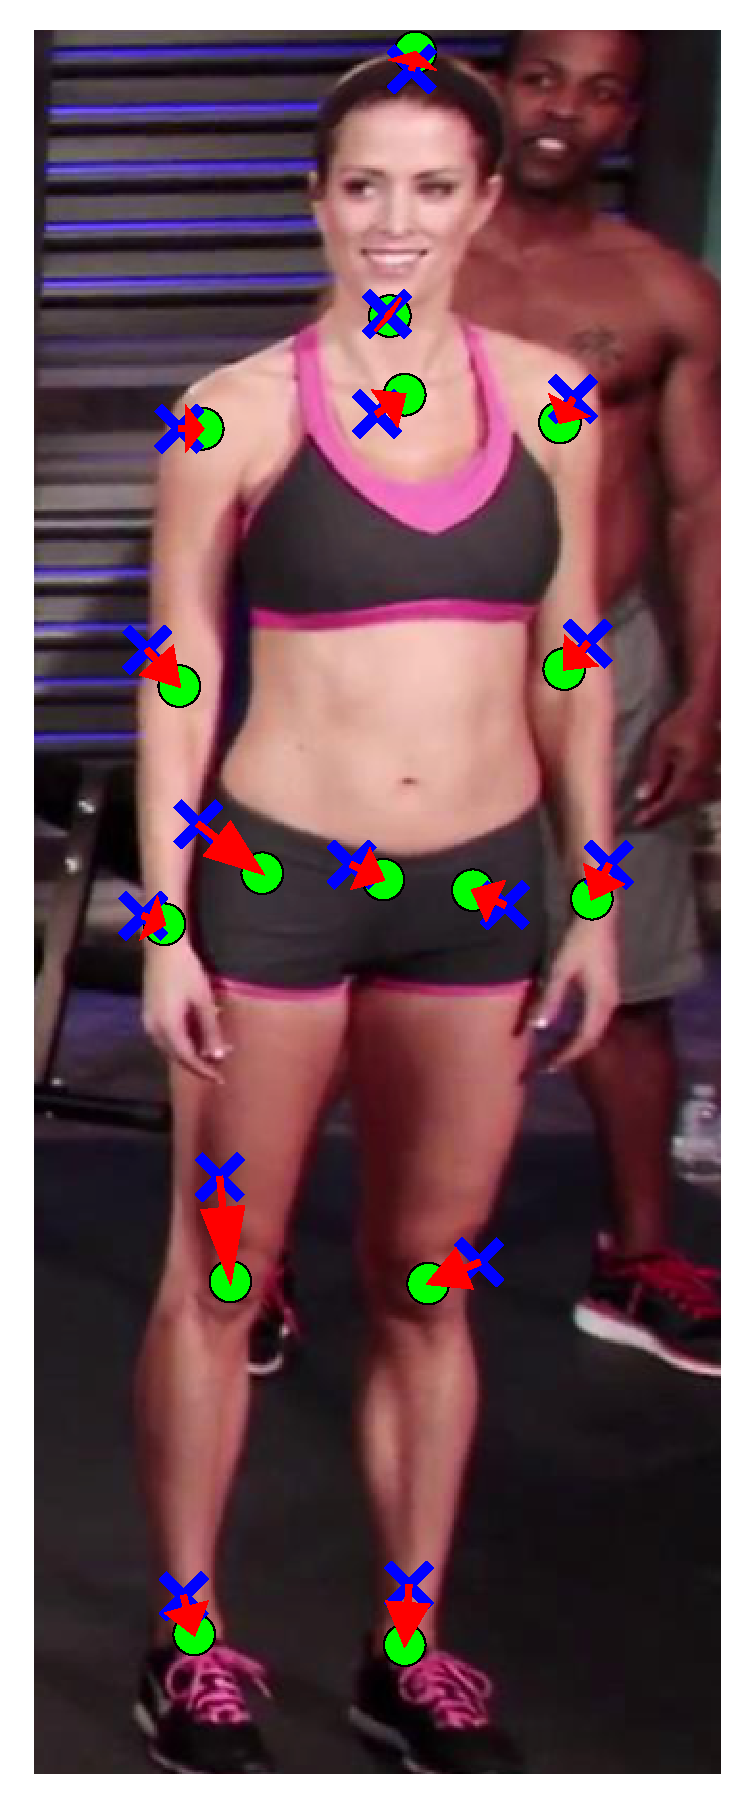
\includegraphics[height=.65\columnwidth]{resources/MotivativeAnnotation/MPII}
        &
        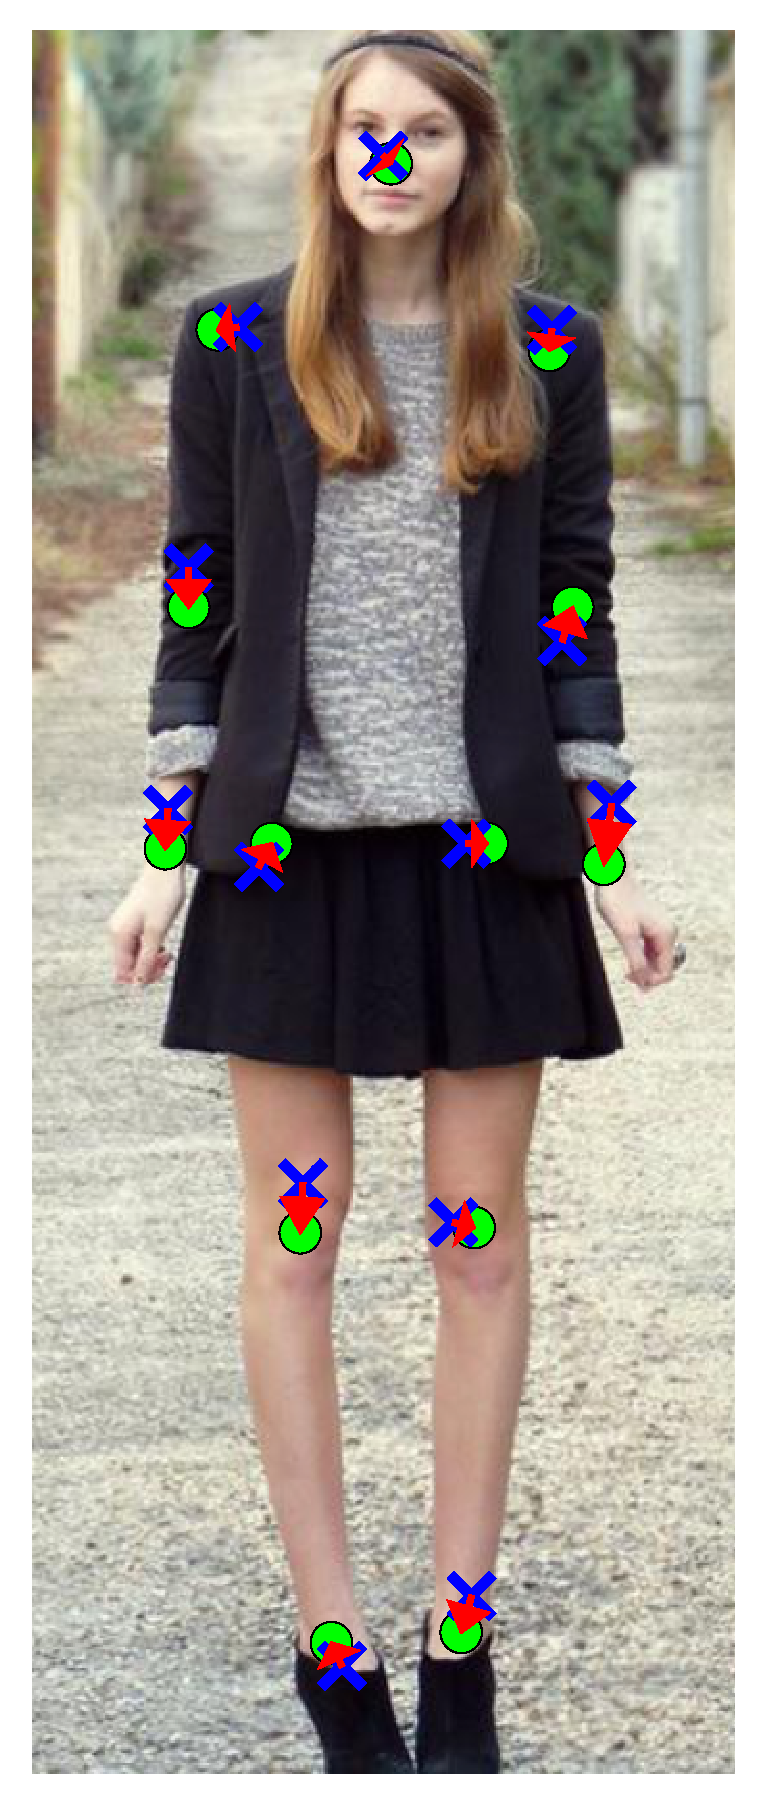
\includegraphics[height=.65\columnwidth]{resources/MotivativeAnnotation/FashionPose}
        &
        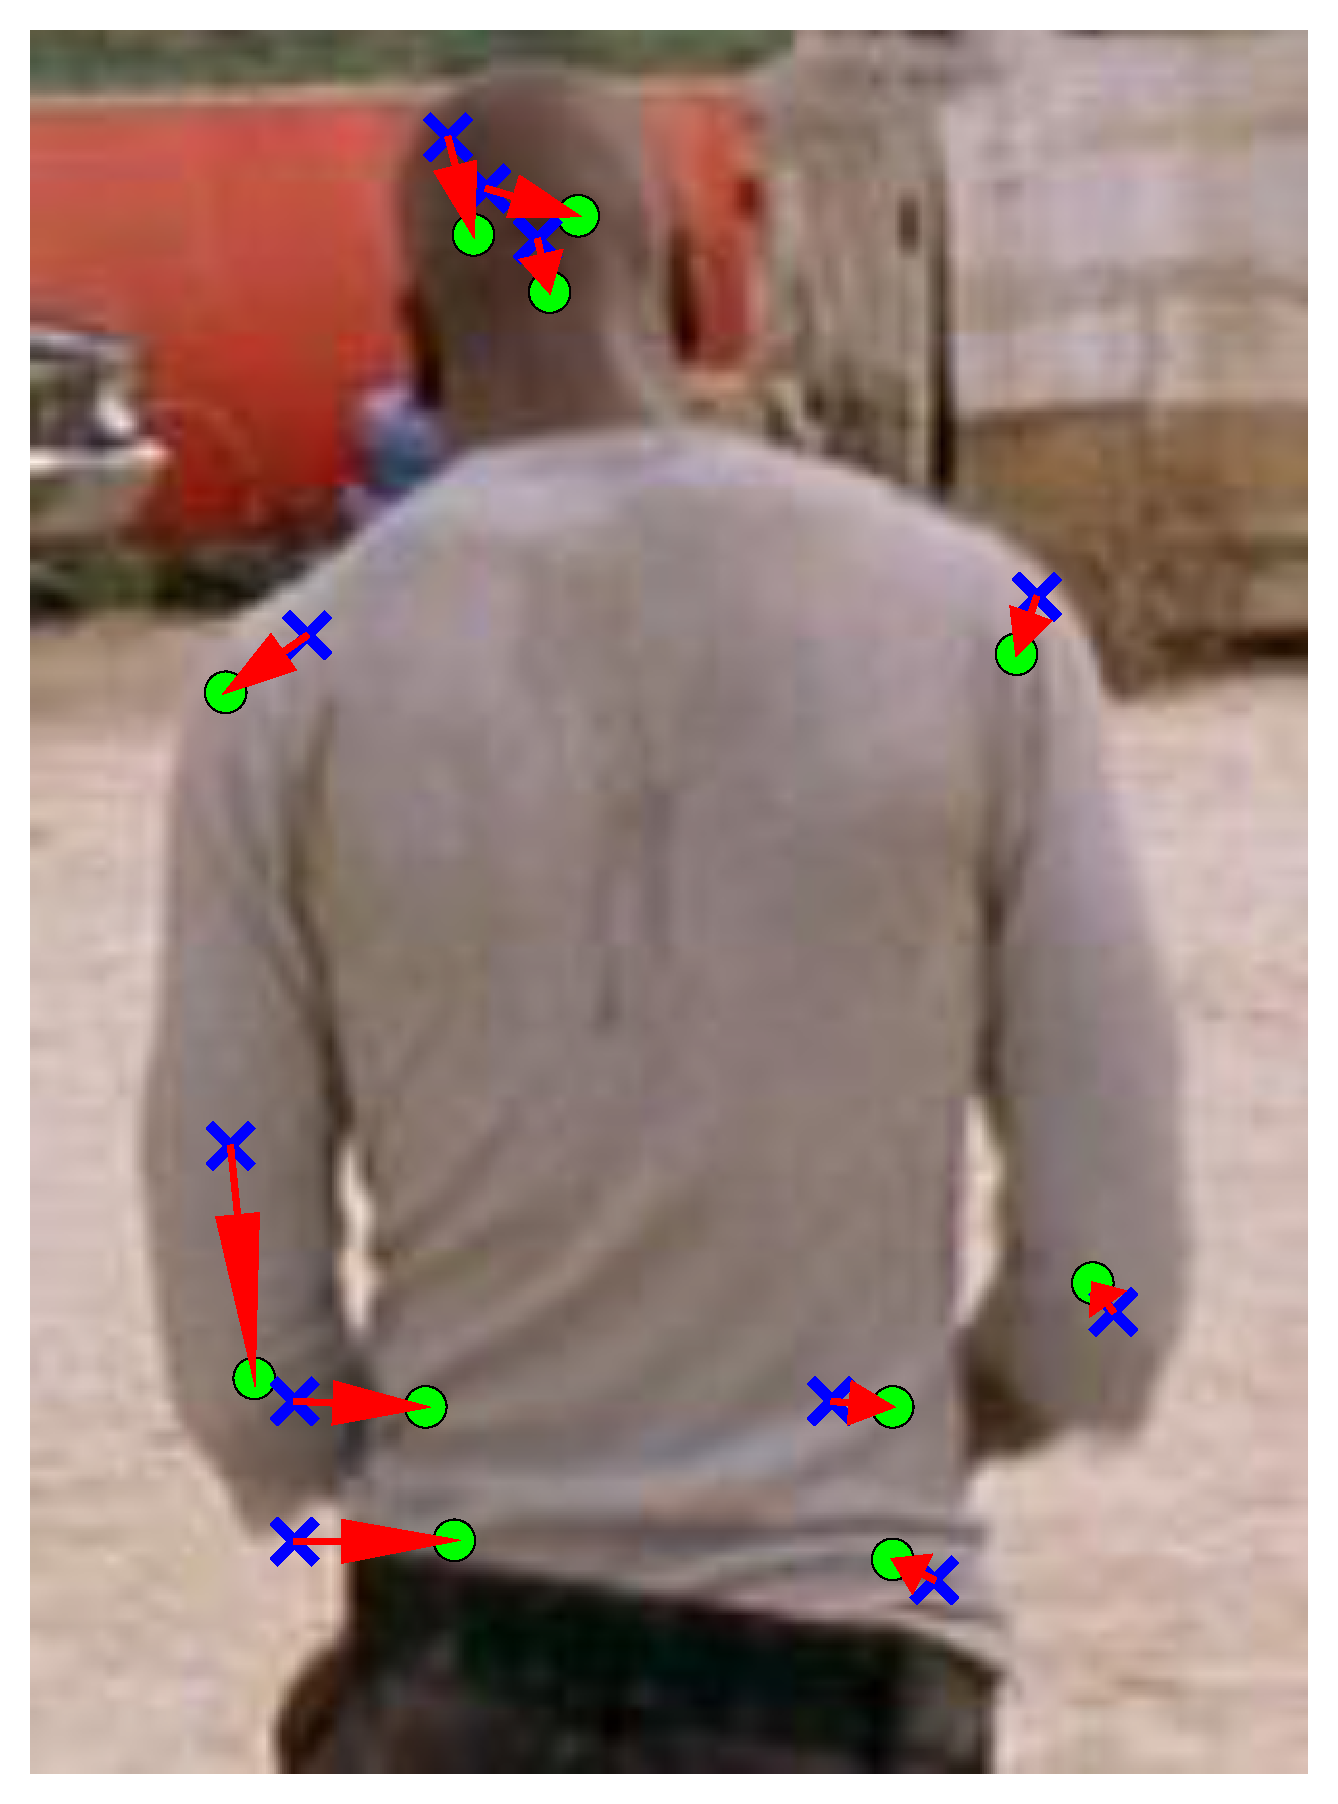
\includegraphics[trim=50 0 50 0,clip,height=.65\columnwidth]{resources/MotivativeAnnotation/FLIC}
        \\
        (a) MPII
        &
        (b) Fashion
        &
        (c) F
        \end{tabular}
    \caption{Examples of inconsistent annotations of human pose among different datasets. \emph{Blue} markers denote the original annotations. The arrows and \emph{green} markers show the correct location at which the points should be annotated.}
    \label{fig:wrong_anno}
\end{figure} 
\begin{figure}[t!]
    \centering
    \begin{subfigure}[b]{0.065\textwidth}
            \includegraphics[height=2.55cm]{resources/Fig_Intro/intro_2_0}
    \end{subfigure}
    \hfill
    \begin{subfigure}[b]{0.065\textwidth}
            \includegraphics[height=2.55cm]{resources/Fig_Intro/intro_2_1}
    \end{subfigure}
    \hfill
    \begin{subfigure}[b]{0.065\textwidth}
            \includegraphics[height=2.55cm]{resources/Fig_Intro/intro_2_2}
    \end{subfigure}
    \hfill
    \begin{subfigure}[b]{0.085\textwidth}
            \includegraphics[height=2.55cm]{resources/Fig_Intro/intro_1_0}
    \end{subfigure}
    \hfill
    \begin{subfigure}[b]{0.085\textwidth}
            \includegraphics[height=2.55cm]{resources/Fig_Intro/intro_1_1}
    \end{subfigure}
    \hfill
    \begin{subfigure}[b]{0.085\textwidth}
            \includegraphics[height=2.55cm]{resources/Fig_Intro/intro_1_2}
    \end{subfigure}
    \\
    \begin{subfigure}[b]{0.156\textwidth}
            \includegraphics[height=2.8cm]{resources/Fig_Intro/intro_0_0}
    \end{subfigure}
    \hfill
    \begin{subfigure}[b]{0.156\textwidth}
            \includegraphics[height=2.8cm]{resources/Fig_Intro/intro_0_1}
    \end{subfigure}
  	\hfill
    \begin{subfigure}[b]{0.156\textwidth}
            \includegraphics[height=2.8cm]{resources/Fig_Intro/intro_0_2}
    \end{subfigure}
    \caption{Comparison of the standard landmark annotation (\emph{red} dots) with the curve annotation (\emph{blue} lines) on arms, ears and faces. It is evident that the curve annotations surpass the inevitable inconsistency of sparse annotations.}
    \label{fig:intro}
\end{figure}


Statistical Deformable Models (SDMs) of various objects is a well-studied and popular area in the intersection of computer vision and machine learning \cite{Cootes1995, Cootes2001, Matthews2004, Saragih2011, Belhumeur2011, Zhu2012, Xiong2013}. Recently, we have witnessed tremendous developments on SDMs of human faces and bodies trained with images that are captured under unconstrained conditions, usually referred to as ``in-the-wild" \cite{Belhumeur2011, Cao2012, Zhu2012, Xiong2013, Asthana2013, Tzimiropoulos2014, Asthana2014, kazemi2014one, Alabort2014, zhu2015face, antonakos2015feature, antonakos2015active, Joan_cvpr2015, tzimiropoulos2015project}. This is attributed to:
\begin{itemize}
\item The abundance of complex visual data, spread through web services (e.g. Youtube, Flickr, Google Images), which has led to the development of ``in-the-wild" databases of human faces and bodies \cite{Belhumeur2011, Le2012, Zhu2012, Burgos2013}.

\item The manual annotation of such databases that has been undertaken by several research teams \cite{sagonas2016faces,charles2013domain,dantone2014body,andriluka14cvpr}.

\item The development of powerful visual features that are able to describe objects and their parts in a robust manner (e.g., SIFT \cite{lowe1999object}, HoGs \cite{Dalal2005}
%and Deep Convolutional Neural Networks \cite{sermanet2013overfeat}
), as well as generative and discriminative methodologies for learning SDMs.
\end{itemize}

However, there are two main drawbacks when building SDMs directly on manually annotated landmarks:
\begin{itemize}

\item Annotating with regards to consistent landmarks is an extremely time-consuming, tedious and labour intensive work \cite{sagonas_iccv_300w_2013}, which is usually performed by a trained person. Furthermore, for various object classes, it requires a highly skilled person in order to identify and annotate landmarks in a consistent manner. For example, the human ear has very complicated inner structures (helix, crus antihelicis, scapha, tragus, lobe etc.) which remarkably differ between different ears. Moreover, certain ear parts, such as fossa triangularies and crus helicis, do not appear in all ears and their visibility is highly sensitive to the head pose and illumination variation. Another such example is the human body, which is generally annotated with regards to a number of landmarks that intuitively correspond to a set of body joints. For most body pose databases, the annotation task was undertaken by a crowd-sourcing Internet marketplace, so-called Amazon Mechanical Turk (AMT). Unfortunately, this resulted in acquiring inconsistent and inaccurate annotations, in many cases\footnote{In the case of faces, the quality of annotations produced from AMT are extremely inaccurate and cannot, by any means, be compared with the ones provided by the recent 300W competition \cite{sagonas_iccv_300w_2013,sagonas2016faces}.} (please see Figure \ref{fig:wrong_anno}). As it was also recently pointed out \cite{tompson2015efficient}, the inconsistencies in body joint annotations may also render the comparison between different human pose estimation methodologies irrelevant.

\item The nature of many deformable objects does not allow them to be annotated with regards to a consistent set of landmarks (e.g., bottles, fruits etc.). Additionally, it is very difficult to consistently annotate the outline of certain objects such as faces, ears, body, since these landmarks do not have any semantic meaning. That is why many state-of-the-art methods opt to leave the boundary out when reporting results \cite{Tzimiropoulos2014, Asthana2014}. The majority of the state-of-the-art methods for model-based landmark localisation \cite{Cao2012, Zhu2012, Xiong2013, Tzimiropoulos2014, Asthana2014} are not applicable to objects with inconsistent sets of landmarks.

\end{itemize}

To illustrate how time-consuming careful annotation of a complex deformable object is, we lay down our own experience based on the human ear. A trained annotator needs an average of 4 minutes per image for the manual annotation of 55 landmarks. This means that the annotation of 1000 images requires a total of about 67 hours. Furthermore, the quality of training as well as fatigue greatly influence the annotation accuracy. Hence, a second pass on the annotated data is, in many cases, necessary. Due to the fact that manual annotation is a costly and labour-intensive procedure, unsupervised learning of deformable models for the task of object alignment has recently attracted some attention \cite{frey2003learning, baker2004automatic, cootes2004groupwise, jojic2006escaping, Huang2006, kokkinos2007unsupervised, jiang2009learning, liu2009simultaneous, Zhang2012}. However, because the problem of fully unsupervised discovery of the deformations of arbitrary objects is difficult and ill-posed, the limited number of methods that have been proposed for the task cannot be directly applied to arbitrary collections of ``in-the-wild" images. On the other hand, the method of \cite{antonakos2014automatic}, which can deal with ``in-the-wild" images, requires a set of consistently annotated sparse shapes to perform deformable face congealing.


\section{Contributions}

In this paper, we propose a solution for annotating an object with regards to its deformations that requires considerably less effort compared to manual annotation and, at the same time, can be used to define statistical deformations for objects without a consistent set of landmarks. We employ the proposed method in order to construct SDMs based on the outline of human body parts (i.e., arms and legs). The proposed SDM can also be used to provide accurate and consistent annotations for several of the body joints (such as wrist, elbow etc.).
To this end, we argue and empirically demonstrate that it is better to annotate an object with regards to a set of continuous lines that describe its shape. An example is provided in Figure \ref{fig:intro}, which compares the standard landmark annotations that are employed in the current literature with the proposed curve annotations for arms, ears and faces. It becomes evident that the curve annotations avoid the inherent ambiguity of placing sparse landmarks and offer a richer description of the object's shape.
%
Furthermore, these curves can be automatically generated by recently proposed methods that perform discriminative segmentation of objects \cite{luo2013pedestrian,liu2015matching}.
%
Note that the work in~\cite{zuffi2012pictorial} is the only one that shows that training SDMs based on the outline contours of the human body parts has considerable advantages compared to using the sparse skeleton joints, as done by the majority of existing SDMs for human pose.

Furthermore, we capitalise on recent advances on multiframe optical flow estimation \cite{Garg:2013hu,tomasi2012dense,snape15faceflow} and show that the relevant methodologies have matured enough to densely annotate the proposed shapes using either simplistic or even more sophisticated and robust shape representation methods \cite{Nguyen2013}.
In particular, in order to build dense correspondences between different shape instances of the same object class, we jointly estimate the optical flow among all the instances by imposing low-rank constrains, an approach that we call \emph{Shape Flow}. Multiframe optical flow has originally been applied on video sequences, relying on the assumptions of colour consistency and motion smoothness \cite{Garg:2013hu}. However, these assumptions do not hold in our case, where we have a collection of shapes. Therefore, we introduce appropriate modifications based on the consistency of image-based shape representation, as well as low-rank priors.


Additionally, we show that the proposed methodology can be applied on landmark localisation, even though it is not tailored for that task, achieving particularly good performance. Specifically, we explain how to build powerful dense SDMs that are suitable for objects that have rich interior texture but lack landmarks consistency. Furthermore, we show how to build a powerful patch-based SDM on the sparse outline landmarks of objects that do not have semantically meaningful interior textures. Using the resulting outline patch-based SDM, we report state-of-the-art performance on the task of human body parts localisation on challenging databases. Finally, we show that the proposed patch-based SDM can be used to provide consistent annotations for different body parts.




In summary, the contributions of this paper are:
\begin{itemize}

  \item We propose one of the first, to the best of our knowledge, methodologies that constructs accurate SDMs from a set of training data with inconsistent annotations. We show that the proposed methodology tremendously reduces the manual workload thanks to the highly effective curve annotations.

  \item We illustrate the ability of the proposed method to generate consistent sparse landmark annotations for object classes which, by nature, make it impossible to be manually annotated in a consistent way.

  \item We show that it is more advantageous to model the human body parts (e.g. arms) with a set of sparse landmarks on their outline, rather than on their skeleton joints. This is because the outline landmarks, which can be acquired by our method in a straightforward way, exhibit better consistency compared to the inevitable inconsistency of the joint landmarks.

  \item We report state-of-the-art quantitative and qualitative results on human body parts localisation by employing a patch-based SDM trained on the outline landmarks that are sampled by the dense correspondences. Our proposed model outperforms all current state-of-the-art techniques that are trained on skeleton joints.

  \item We show that the employed patch-based SDM corrects the annotations that are currently provided for most major human body pose databases \footnote{\label{foot:annotations}The corrected annotations are publicly available in \url{http://www.ibug.doc.ic.ac.uk/resources/bodypose-anno-correction}.}.

\end{itemize}



%In our experiment, we show that building robust dense models trained with inconsistent annotation and %trained with curve annotation improves performance of discriminative models trained on carefully %annotated data including ears, faces, bottles, (cars ?) and bodies. Evaluation methods and choices are %described in details.




%We propose a framework to (1) construct SDMs using training data with inconsistent annotation, (2) %introduce highly effective curve annotation which tremendously reduces manual work overload but %maintains same performance level against state-of-the-art SDMs and (3) build dense correspondent SDMs %with shape flow.

%(1)
%Annotated data of same objects can have various number of landmarks, \cite{?} shown faces have %landmarks different in range 10+ to 70+. Building SDMs (e.g. Active Appearance Models), however, %%require training data are annotated consistently, for example, all faces have 68 landmarks, 6 landmarks %for an eye and 9 for a nose \cite{?}. Such property of SDMs largely limited their application area like %combining different dataset as one. We propose the pipeline with non-rigid alignment and support vector %shape to blend landmarks into relatively consistent shape discriminator before building models.

%(2)



%(3)


% Back Ground, uses Nondas' paper "Automatic Construction of Deformable Models In-The-Wild" as place holder
%The two most closely related works to the proposed
%method are the automatic construction of Active Appearance
%Models (AAMs) in \cite{?} and the so-called RASL
%methodology in \cite{?} for person-specific face alignment.
%There are two main differences between our framework
%and \cite{?}. (1) We use a predefined statistical shape model
%instead of trying to find both the shape and appearance models.
%We believe that with the current available optimization
%techniques, it is extremely difficult to simultaneously optimize
%for both the texture and shape parameters. (2) We
%employ the robust component analysis of \cite{?} for the appearance
%which deals with outliers. Thus, even though
%our method is similar in concept to \cite{?}, these two differences
%make the problem feasible to solve. In particular, the
%methodology in \cite{?} fails to create a generic model even in
%controlled recording conditions, due to extremely high dimensionality
%of the parameters to be found and to the sensitivity
%of the subspace method to outliers. This was probably
%one of the reasons why the authors demonstrate very
%limited and only person-specific experiments. Furthermore,
%our methodology bypasses some of the limitations of \cite{?},
%which requires the presence of only one low-rank subspace,
%hence it has been shown to work only for the case of congealing
%images of a single person. Finally, we argue that
%in order for an automatically constructed AAM methodology
%to be robust to both within-class and out-of-class outliers4,
%which cannot be avoided in totally unsupervised setting
%statistical component analysis techniques should be
%employed \cite{?}.


\begin{figure*}[t!]
    \centering
        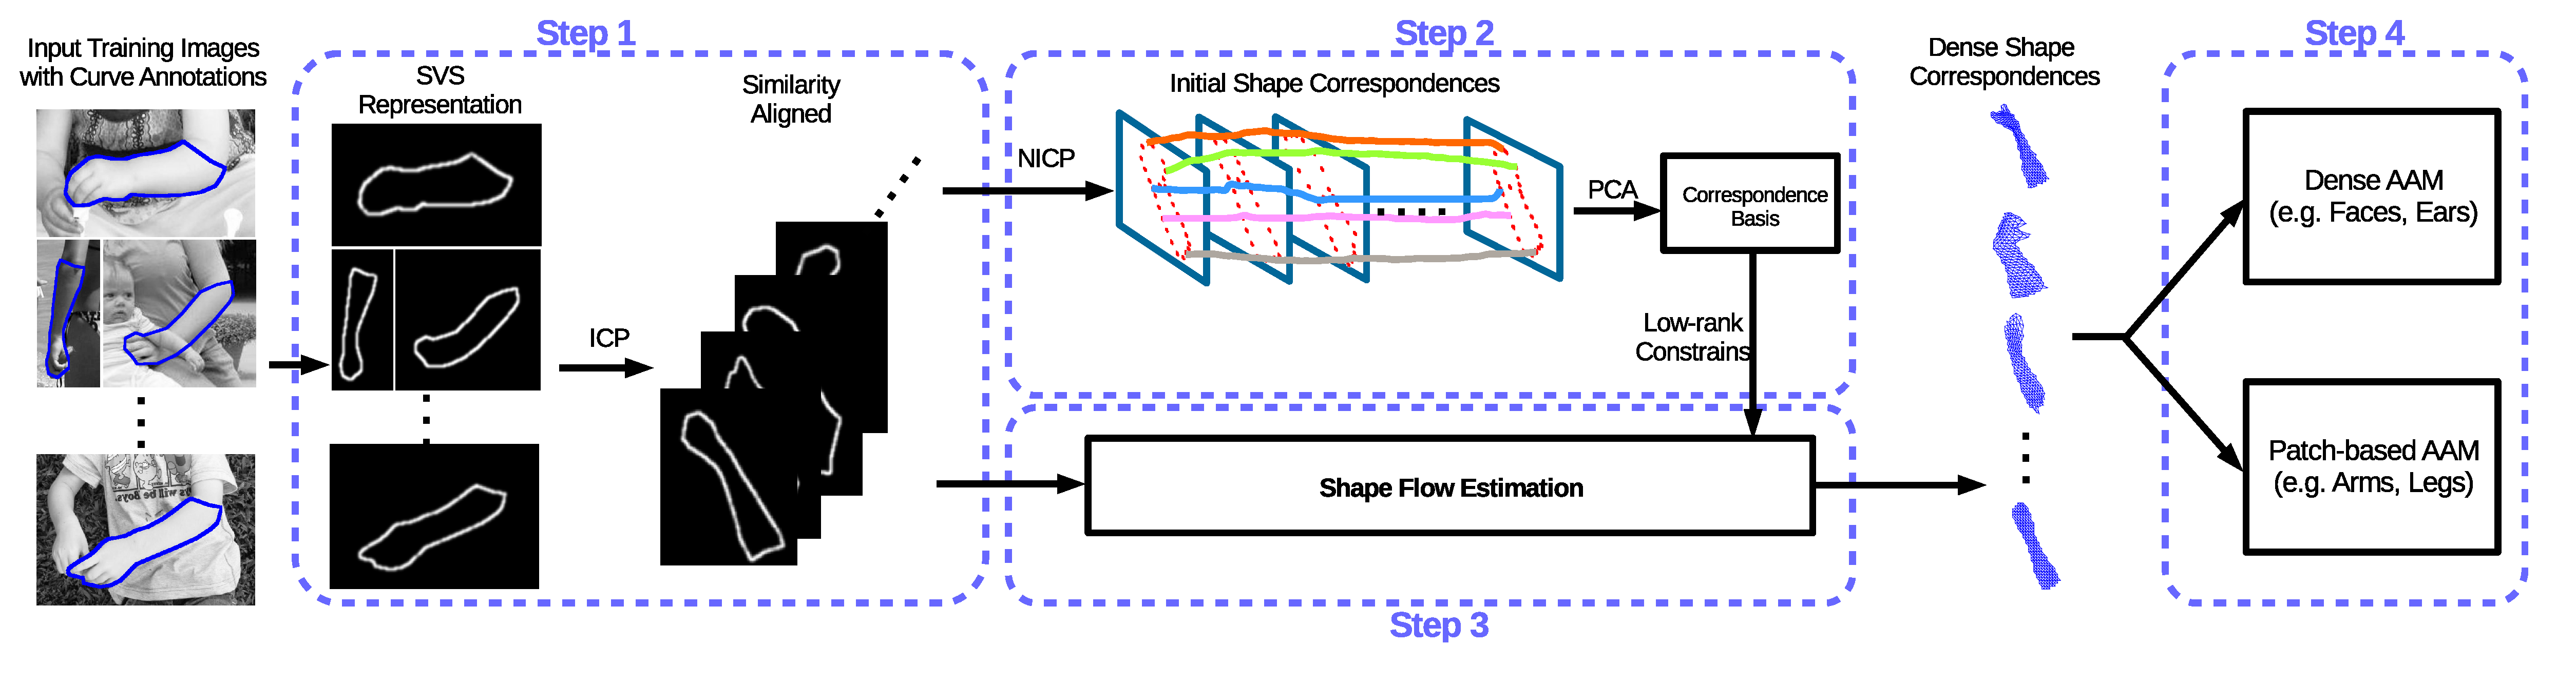
\includegraphics[width=\textwidth]{resources/architecture3}
    \caption{Schematic description of the proposed pipeline. Figure best viewed by zooming in.}
    \label{fig:archi}
\end{figure*}

\section{Constructing Deformable Models with Shape Flow}

% Deformable models are widely used for object detection, localization, recognition and tracking while training a deformable model with good generalisation requires tremendous amount of carefully annotated data, which is extremely time consuming. Even more, annotated data of a specific object category typically requires same numbers of landmarks for every training sample, making the annotation procedure significantly complex where corrext menual annotation of landmarks is impossible in various object classes e.g. ears.

% Despite the fact that that vast majority of existing methods are based on a sparse shape representation, dense shape representation reveals more nuanced structure in terms of [todo: explain].


This section presents the proposed method for establishing dense correspondences among training shapes
by only using curve annotations.
%
%We propose a novel framework for building deformable models that does not require any consistent set of annotated landmarks and is based on a dense shape representation. Our method only requires a set of point or curve line annotations that does not need to be consistent over different training samples.
%
%It combines the techniques of Non-rigid Iterative Closest Point (NICP) \cite{Amber2007}, multichannel Support Vector Shape (SVS) \cite{Nguyen2013} representation and multiimage subspace flow \cite{Garg:2013hu} in an effective framework that has significant descriptive power.
%
It takes as input a set of training images of a particular object class, along with the corresponding curve annotations. The steps of our pipeline, which are also depicted in Figure~\ref{fig:archi}, are the following:

\noindent\textbf{Step 1:} Represent the curve annotations in a consistent way using a multichannel extension of the Support Vector Shape (SVS) representation \cite{Nguyen2013}. Apply the Iterative Closest Point (ICP) algorithm \cite{Besl1992} to achieve an initial alignment of the SVS images.

\noindent\textbf{Step 2:} Construct a correspondence basis for the training SVS images. This is acquired by applying the Non-rigid ICP (NICP) algorithm of \cite{Amber2007} on the densely sampled annotated curves, followed by Principal Component Analysis (PCA).

\noindent\textbf{Step 3:} Establish dense correspondences between all the shapes in the training set by feeding the multichannel similarity-aligned SVS images into a multi-image subspace flow estimation.

\noindent\textbf{Step 4:} Utilise the dense correspondences acquired by the optical flow in order to automatically generate either dense or sparse (on the outline) landmark annotations, depending on the object class type. Then, build either a dense \cite{ramnath2008increasing, Amberg2009, anderson2014using} or a patch-based \cite{Tzimiropoulos2014} AAM, respectively.

The upcoming sections discuss each of the aforementioned steps in further detail.

%two major modules. The first module handles inconsistent annotation set by converting to landmark independent shape discriminator. While the other module produces shape flow on object discriminators to generate dense flow transformations in shape space following by robust PCA\cite{?} to generate deformable model. In this section, we present the entire architectures, design decision and algorithms.
\newcounter{steps}
{\refstepcounter{steps}\label{sec:step1}\subsection*{Step 1: Shape Representation Based on Support Vector Shapes}}
% \subsection{Shape Representation Based on Support Vector Shapes}
% \label{sec:step1}
%Ordinarily, construction of deformable model requires training data set having consistent number of landmarks. But unavoidable changes has to be made before applying same algorithm on diverse annotated data set.

In order to fully capture the variability among most deformable objects' shapes annotations, we use a representation based on SVS \cite{Nguyen2013}. An SVS is a decision function trained on shapes using Support Vector Machines (SVMs) with Radial Basis Function (RBF) kernels. In this way, a shape is represented as a classifier function, which has several advantages: (a)~the representation is completely generic, e.g. it can be applied to sparse landmark points, curves lines or a combination of the two, and~(b) it fuses inconsistent landmarks into consistent and directly comparable decision functions. Furthermore, this representation is also robust against noise, missing data and outliers \cite{Nguyen2013}.

%In practice, we assume that all the training images correspond to the same object category and contain a set of inconsistent points and curve line annotations.
The curve annotations for all training images are densely sampled to yield a set of landmarks per image, with this set being different for every training image. To train the SVM, these landmarks are assigned as belonging to the `positive' class, whereas randomly sampled points around them are assigned as belonging to the `negative' class. Since the positive class has far less points than the negative class, landmarks are assigned considerably larger weights so that $N_p \times W_p=N_n \times W_n$ where $N_p, N_n$ are number of points of the positive and negative class respectively and $W_p, W_n$ are their corresponding weights.

SVMs with RBF kernel functions map any number of data points onto an infinite-dimensional space where positive and negative points are linearly separable, hence the classification boundary on the 2D space represents the actual shape of the object.
%Note that the decision function for SVMs can be mathematically expressed as:
%\begin{equation} \label{eq:decisionfunc}
%    d(\bm{x})=\sum_i\alpha_i \, k(\bm{x}_i^*,\bm{x})
%\end{equation}
%where $\bm{x}_i^*$ are the so-called support vectors and \mbox{$k(\bm{x}, \bm{y}) = \exp(-{\|\bm{x} -\bm{y}\|^2}/{2 \sigma^2})$} is the RBF kernel.
Let $d(\bm{x})$ be the decision function for SVMs. In our formulation, $d(\bm{x})$ can be defined for every pixel $\bm{x}$ of the corresponding object image, therefore we interpret it as an image and we call it \emph{SVS image}.

%Figure~\ref{fig:archi} includes some exemplar SVS representations of arm shapes (Step 1 box)

%Figure \ref{fig:build_svs} shows an exemplar shape representation of the human ear using SVS. As it can be observed, the final result does not drastically depend on the original number of annotated landmarks.


% \begin{figure}[b!]
%     \centering
%     \begin{subfigure}[b]{0.2\textwidth}
%             \includegraphics[width=\textwidth]{resources/landmark}
%         \caption{Spare landmarks}
%     \end{subfigure}
%     \qquad
%     \begin{subfigure}[b]{0.2\textwidth}
%             \includegraphics[width=\textwidth]{resources/svs}
%         \caption{Decision function}
%         \label{fig:svs}
%     \end{subfigure}
%     \caption{Exemplar SVS shape representation. The decision function is trained on the set of sparse landmarks. In (b), brighter colour represents higher probability of a pixels belonging to the original shape.}
%     \label{fig:build_svs}
% \end{figure}

% \begin{figure}[b!]
%     \centering
%     \includegraphics[width=0.4\textwidth]{resources/svs2}
%     \caption{Exemplar SVS shape representation. A similar SVS image is obtained from different annotations of the same shape.}
%     \label{fig:build_svs}
% \end{figure}

We extend the SVS representation to support also the case where multiple curves with different labels are annotated. This is useful when annotating different structures of the same object, such as the left and right eyebrows on faces. Even though not absolutely necessary in our framework, it can provide further guidance on the estimation of dense shape correspondences for various object classes. In more detail, we create a multichannel SVS image $\bm{d}(\bm{x})=[d_1(\bm{x}) \cdots d_i(\bm{x}) \cdots d_{N_c}(\bm{x})]$, where $d_i(\bm{x})$ is the SVS image that corresponds to the curve annotation of the $i$-th structure and $N_c$ is the total number of structures (a single curve annotation is the special case where $N_c=1$). Note that we do not necessarily require that all structures are annotated in all the object images: in the case that a structure is not annotated, the corresponding channel of the SVS image simply takes a zero value for all pixels. The shape flow estimation can deal with such missing information thanks to the spatial regularization and the low-rank constraint that it adopts, c.f.~Step~\ref{sec:step3}.

After constructing the SVS representation for all images, the next step is to apply a simple similarity alignment over them. This is done because the goal here is to build a model capable of effectively representing non-rigid local shape deformations rather than global rotation, translation and scaling. The alignment is performed by using the ICP algorithm \cite{Besl1992} on the annotated landmarks point cloud of the training images.


\vspace{0.2cm}
%\subsection{Correspondence Basis for Shape Flow Estimation}
{\refstepcounter{steps}\label{sec:step2}\subsection*{Step 2: Correspondence Basis for Shape Flow Estimation}}

We define the problem of shape flow as the joint estimation of optical flow fields between a reference SVS image and every SVS image of the training dataset, which yields dense correspondences across SVS images. This also defines for every training SVS image a warping function that registers it with the reference SVS image. To establish the dense correspondences robustly, we are inspired by the idea of subspace constraints in the estimation of multiframe optical flow \cite{Garg:2013hu,tomasi2012dense,snape15faceflow}.

Instead of the \emph{motion} basis used in multiframe optical flow formulation of \cite{Garg:2013hu}, we build a \emph{correspondence} basis that introduces constraints on how points of different shapes are matched to each other. Every pixel of the reference SVS image is matched to its corresponding position at every training SVS image and in this way defines a \emph{correspondence vector}. This vector consists of the 2D locations of the specific point in all SVS images. To form this vector, the training images are arranged in an arbitrary order. Similarly to the order of the training samples when PCA is applied, this order does not affect the result of our method and any re-ordering would produce exactly the same results.


Formally, let $N_t$ be the number of training SVS images and $n=1,\ldots,N_t$ be the training image index. Also, let $\boldsymbol{q}_1(n),\ldots,\boldsymbol{q}_R(n):\{1,\ldots,N_t\} \rightarrow \R^2$ be the $R$ orthonormal elements of the correspondence basis, where $\boldsymbol{q}_i(n)$ is the displacement vector that matches the points of the reference SVS image with the points of the $n$-th training SVS image, according to the variation described from the $i$-th correspondence basis element. Note that the basis elements $\boldsymbol{q}_i(n)$ are independent from the point location. Note also that the number of basis elements is typically much smaller than the full dimensionality ($2 N_t$) of correspondence vectors, therefore this basis plays a role of dimensionality reduction. 


In addition, let $\Omega \subset \R^2$ be the image domain of the SVS images and $\bx$ denote the point location. We denote the shape flow result as $\bm{u}_n(\bx):\Omega\times \{1,\ldots,N_t\}
\rightarrow \R^2$,  where $\bm{u}_n(\bx)$ is the displacement vector that matches the point $\bx$ of the reference SVS image with its corresponding location at the $n$-th training SVS image.

Using the constructed correspondence basis, the shape flow can be approximated as:
\vspace{-5pt}
\begin{equation}\label{eq:LinTrajModel}
    \bm{u}_n(\bx) \approx
    \textstyle \, \sum_{i=1}^R \, \bm{q}_i(n)v_i(\bx) \,\, ,
\vspace{-5pt}
\end{equation}
where $v_i(\bx)$ is the weight that needs to be applied on the $i$-th correspondence basis element, in order to get the correspondence vector for the point location $\bm{x}$. In other words, the shape flow for every point $\bm{x}$ is described as a linear combination of basis elements that is controlled by the coefficients $v_i(\bm{x})$.
The values of the $i$-th coefficient for all the points $v_i(\bm{x})$ can be interpreted as an image defined on $\Omega$. Using the correspondence basis, the determination of the shape flow boils down to the determination of the set of coefficients $v_i(\bm{x})$. The above representation of shape flow, constrains the correspondence vectors to lie on a subspace and, therefore, acts as a low-rank prior that enforces coherency of the shape registration result over the whole training dataset of shapes.


To effectively build the correspondence basis, we first transform the original annotations to sparse point clouds. Then, we apply the NICP algorithm of \cite{Amber2007} between the point cloud of annotations in the reference shape and the one of every shape of the training set. NICP iteratively deforms the cloud of points of every shape to match the points of the reference shape. This yields an initial estimation of the correspondence vectors on the sparse locations of annotated landmarks on the reference shape. Finally, the correspondence basis is found by applying PCA on these correspondence vectors and keeping only the first $R$ principal components.



% For all dense transformations $\bm{u}_n(\bm{x}), n \in \{1,...,F\}$, where $F$ is number of data and $\bm{x}$ is vector of pixels, Principle Component Analysis (PCA) is performed on trajectory to obtain low rank trajectory basis:
% \begin{equation}
%     \begin{bmatrix}
%         \bm{u_1}(\bm{x}) \\
%         \vdots \\
%         \bm{u_F}(\bm{x})
%     \end{bmatrix}
%     =
%     \begin{bmatrix}
%         \bm{q_1}(1) & \cdots & \bm{q_R}(1) \\
%         \vdots      & \ddots & \vdots  \\
%         \bm{q_1}(F) & \cdots & \bm{q_R}(F)
%     \end{bmatrix}
%     \times
%     \begin{bmatrix}
%         \bm{v_1}(x) \\
%         \vdots \\
%         \bm{v_R}(x)
%     \end{bmatrix}
% \end{equation}
% where $\bm{q_i}(n)$ are low rank components with $R \ll 2F$ and $\bm{v_i}(x)$ weighted each component with dependencies on $x$. Simpler expression shown below:
% \begin{equation}
%     \bm{u}_n(\bm{x})=\sum_{i=1}^R\bm{q_i}(n)\bm{v_i}(x)+\bm{\varepsilon_n}(\bm{x})
% \end{equation}

\begin{figure}[t!]
    \centering
    \newcommand{\flowh}{0.25\columnwidth}
    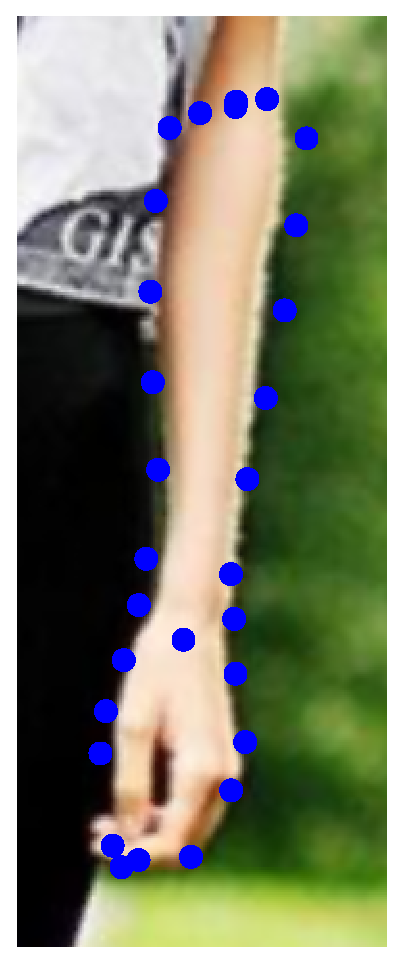
\includegraphics[height=\flowh]{resources/Fig_Flows/1}
    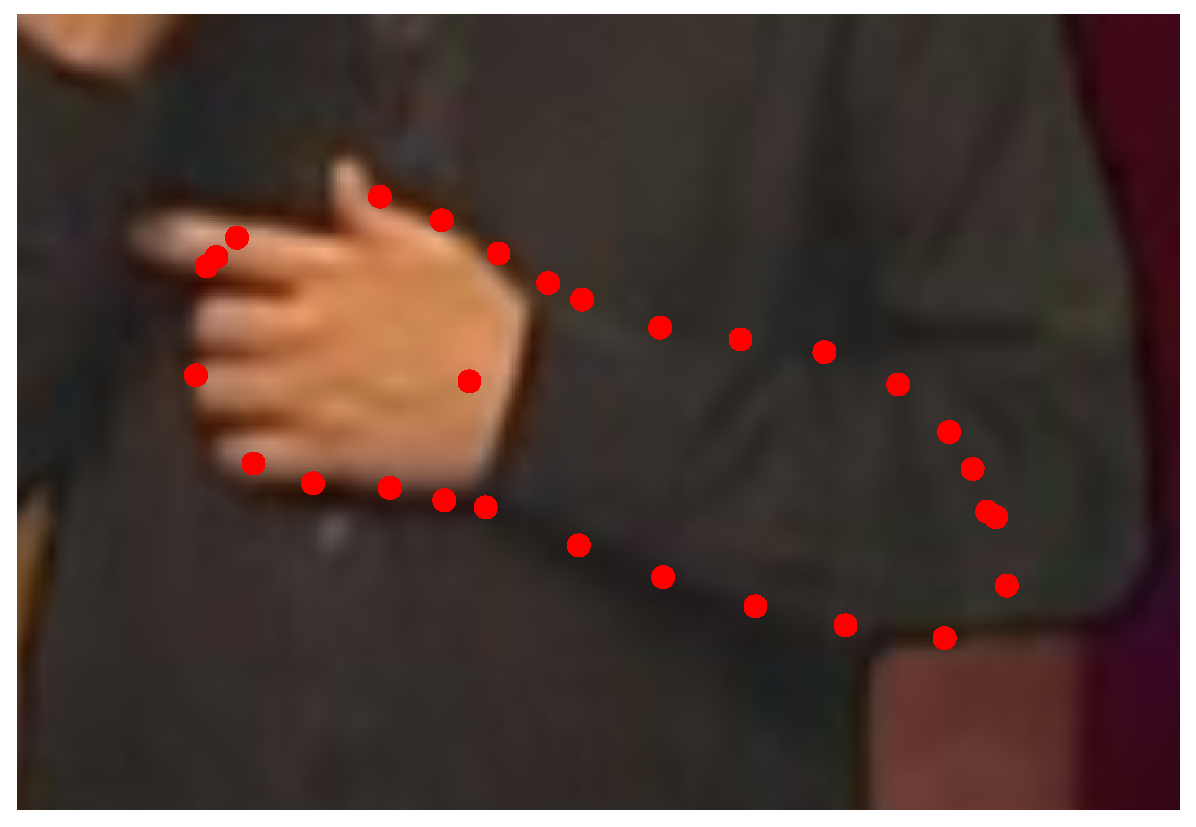
\includegraphics[height=\flowh]{resources/Fig_Flows/2}
    \includegraphics[height=\flowh]{resources/Fig_Flows/3}
    \includegraphics[height=\flowh]{resources/Fig_Flows/4}
    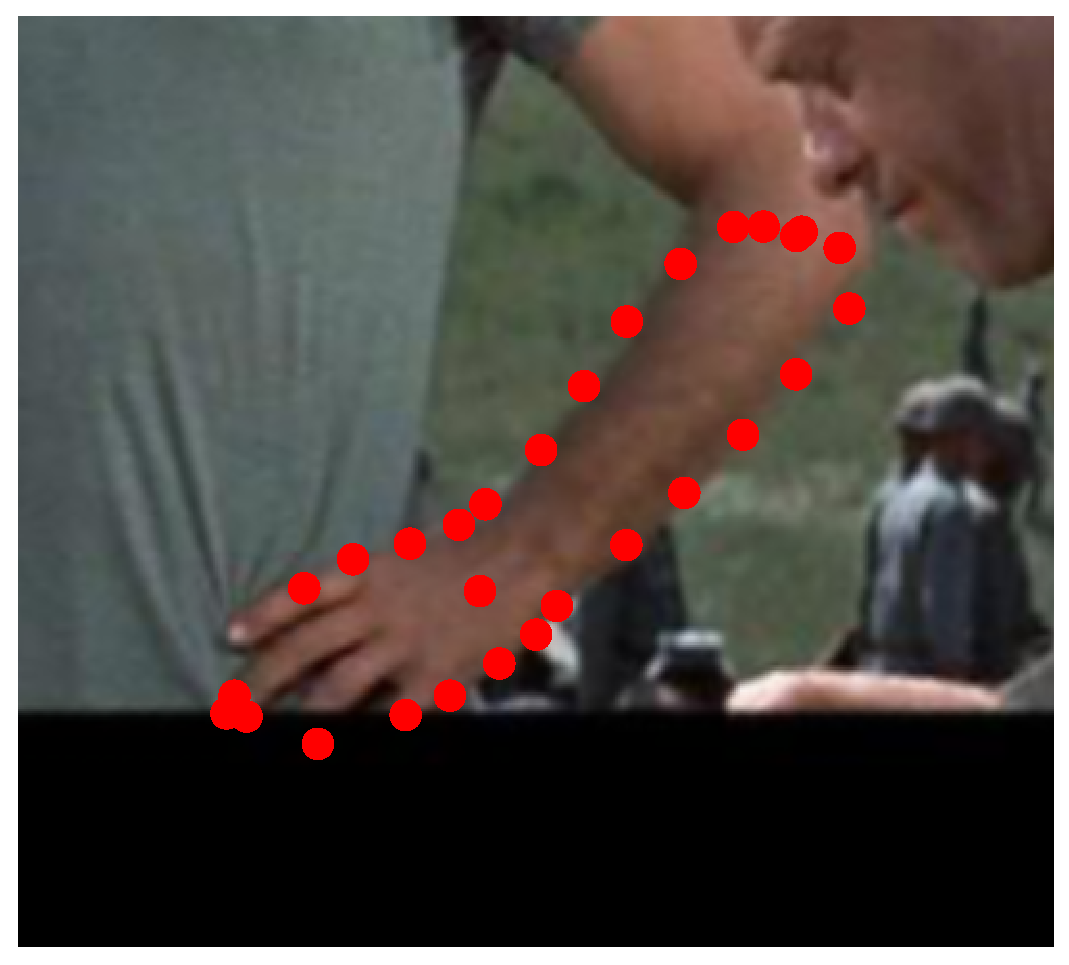
\includegraphics[height=\flowh]{resources/Fig_Flows/5}
    \includegraphics[height=\flowh]{resources/Fig_Flows/6}
    \caption{Exemplar deformation fields for the left arm, obtained using the proposed pipeline. Figure best viewed by zooming in.}
    \label{fig:deformationfield}
\end{figure}

\begin{figure}[b!]
    \centering
    \includegraphics[width=0.9\columnwidth]{resources/models}
    \caption{Dense shape models build for faces and ears. Dense shapes are presented as grid for better visualization.}
    \label{fig:dense_models}
\end{figure}




% ---------------------------------------------------------------------------------------------------------------------------------------------------
\vspace{0.3cm}
{\refstepcounter{steps}\label{sec:step3}\subsection*{Step 3: Shape Flow Estimation}}
% \subsection{Shape Flow Estimation}
% \label{sec:step3}


%Using the SVS functions built from training data, one of the main steps of our pipeline is to estimate dense correspondences between all these functions. We propose to perform this estimation simultaneously for all training data, by using the correspondence basis.

As already mentioned, our shape flow estimation builds upon robust methods for multiframe optical flow estimation \cite{Garg:2013hu}. However, optical flow estimation typically works based on the assumptions of brightness or colour constancy and motion smoothness, whereas in our setting the input training data correspond to shapes. For this reason, we propose to modify the formulation of \cite{Garg:2013hu} by using the correspondence basis that we introduced in conjunction with the SVS representation of shapes.


%
%In order to learn the such a subspace, we first transform the original annotation to point clouds. Then, we use NICP to align the previous point clouds with respect to a reference point cloud template. NICP iteratively deforms each point cloud until its points match the ones on the shape template and correspondences are established. However, because optical flow is a pixel-wise frame registration technique, we need to establish correspondences for all pixels on the reference frame rather than for sparse point clouds. To achieve this, we apply Thin Plate Spline (TPS) \cite{Bookstein1989} to find correspondences for all pixels in the reference frame given the point cloud correspondences provided by the previous NICP stage. Once dense correspondences have been established among all pixels, the so-called correspondence subspace is obtained by performing PCA the trajectory of all pixels. Note that incorporating the previous subspace as a low rank constrained in optical flow is consistent with its assumption of smooth motion.


Let $\bm{d}(\bx;n)$, $\bm{d}(\bx;0):\Omega\rightarrow \R^{N_c}$ be the $n$-th training SVS image and the reference SVS image respectively. Following \cite{Garg:2013hu}, we propose to estimate the shape flow over all training images by minimizing the following energy:
\vspace{-5pt}
\begin{align}
E_{sf} & =\alpha
\int_{\Omega}\sum_{n=1}^{N_t} \|\bm{d}(\bx+\bm{u}_n(x);n)-\bm{d}(x;0)\| \ud \bx \label{eq:costfunc}\\
    &+ \beta \int_{\Omega}\sum_{n=1}^{N_t}\|\bm{u}_n(\bx)-\sum_{i=1}^R\bm{q}_i(n)v_i(\bx)\|^2 \ud \bx \label{eq:lowrank}\\
    &+
\int_\Omega  \sum_{i=1}^R \,\, \left \|    \nabla v_i(\bx)    \right \|  \,\ud \bx \label{eq:TVterm}
\vspace{-5pt}
\end{align}
This energy consists of two sets of unknown shape flows that are relatively close to each other: (i) $\bm{u}_n(x)$ which tries to explain the data from the input SVS images, and (ii) the shape flow determined by the correspondence basis coefficients $v_i(\bx)$ that are spatially regularised and enforce a low-rank prior.
%We minimize this energy jointly with respect to $\bm{u}_n(\bx)$ and $v_i(\bx)$.
%The positive parameters $\alpha$ and $\beta$ weigh the balance between the terms of the energy.


The \textbf{first term} of the above energy \eqref{eq:costfunc} is a data attachment term
that uses the robust $\Lone$-norm.  It is based on the assumption that the values of the reference SVS image $\bm{d}_0(\bx)$ at every pixel $\bx$ are preserved at its corresponding locations on all training SVS images $\bm{d}_n(\bx)$. The use of an $\Lone$-norm improves the robustness of the method since it allows deviations from this assumption, which might occur in practice.
The \textbf{second term} of the energy \eqref{eq:lowrank} penalizes the difference between the two sets  of shape flows and acts as a coupling term between them.
The \textbf{third term} of the energy \eqref{eq:TVterm} corresponds to the spatial Total Variation regularization \cite{rudin92} of
the correspondence basis coefficients $v_i(\bx)$.
This term penalizes spatial oscillations of each coefficient caused by distortions of the SVS images but not strong discontinuities that are desirable in the borders of different object regions. In addition, this term allows to fill in information into regions where the shape information in the SVS images is missing, due to e.g.~regions with no annotations.

We implement the minimization of the energy $E_{sf}$ by using the optimization algorithm described in \cite{Garg:2013hu}. For more details, please refer to the Supplementary Material.
%We slightly modify this algorithm so that, instead of initialising the coarse-to-fine and warping iterations with a zero flow, we use Thin Plate %Splines (TPS) \cite{Bookstein1989} interpolation of the initial correspondence vectors described in Step~\ref{sec:step2}.
%This yields a significantly better initial location of the highly-nonconvex objective function and improves the computational efficiency, since much less coarse-to-fine pyramids are needed.
%
Figure~\ref{fig:deformationfield} shows some examples of deformation fields derived from the estimated shape flow computed by the aforementioned method. These results correspond to exemplar training shapes in the case of an arm dataset. We observe that the shape flow estimation captures the shape and deformations of the human arm in a plausible way.

%In every coarse-to-fine and warping iteration, we use an initialization that comes from the previous iteration and for the very beginning, we initialize with a Thin Plate Splines (TPS) \cite{Bookstein1989} interpolation of the initial correspondence vectors described in Sec.~\ref{sec:step2}. We approximate the data term \eqref{eq:costfunc} by linearizing the SVS images around the initialization. After that, the energy becomes convex and we optimize it using alternating optimization w.r.t.~$v_i(\bx)$ and $\bm{u}_n(\bx)$. The minimization w.r.t.~
%$v_i(\bx)$ is decoupled for every coefficient $i$ and corresponds to Rudin-Osher-Fatemi Total Variation denoising \cite{rudin92}, which we solve efficiently by applying the first order primal-dual algorithm of \cite{Chambolle:Pock:JMIV2011}. The minimization w.r.t.~
%$\bm{u}_n(x)$ is decoupled for every pixel $\bx$ and every shape index $i$. This minimization is also implemented by applying the efficient primal-dual algorithm of \cite{Chambolle:Pock:JMIV2011}.






%
%
%To register all decision functions to temp`late shape, decision function $d_i(\bm{x}), i \in {1,...,F}$ are grouped into one sequence before applying flow algorithm. The objective cost function we would like to minimise is:
%\begin{align}
%    \operatorname*{arg\,min}_{\bm{u}_n(\bm{x}), \bm{v}}&=\alpha \int_{\Omega}\sum_{n=1}^F|\bm{d_n}(x+\bm{u}_n(x))-\bm{d_0}(x)\| dx  \label{eq:costfunc}\\
%    &+ \beta \int_{\Omega}\sum_{n=1}^F\|\bm{u}_n(x)-\sum_{i=1}^R\bm{q_i}(n)\bm{v_i}(x)\|^2 dx \label{eq:lowrank}\\
%    &+ \sum[\bm{TV}(Qv)]
%\end{align}
%where $d_n(x)$ is the decision function from~\eqref{eq:decisionfunc}, which returns possibilities of given coordinate classified as shape component where coordinates are from set $\Omega \in \Re^2$. $TV(Qv)$ is total variation as regularization on low rank subspace, $Q$ is trajectory basis and $v^T.L.v$ is low rank spacial constrains.
%
%Term~\eqref{eq:costfunc} state the shape constancy where points having similar classification probability are from same object.
%Part~\eqref{eq:lowrank} applies constrain on low rank trajectory basis states in section~\ref{sec:trabasis}.
%The objective cost function has two free parameters $u$ and $v$, so we perform alternating minimisation. The equation can be solved using a thresholding scheme after linearisation of image functions. The minimisation can be speed up by paralleling the minimisation for every spatial-temporal point $(x;n), x \in \Omega, n \in \{1,...F\}$ independently.
%
%
%
%
%
%
%After solving the equation, $\bm{u}_n(\bm{x}), x \in \Omega$ gives a group of deformation fields that registering every decision functions in the shape sequence to reference frame e.g. $\bm{u_1}(\bm{x})$ registers decision function $\bm{d_1}(\bm{x})$ to the reference frame. Figure~\ref{fig:deformationfield} demonstrates deformation fields that warps from reference frame where there is no deformation.

% \begin{figure}[h!]
%     \centering
%         \includegraphics[width=0.5\textwidth]{resources/df}
%     \caption{Deformation field built}
%     \label{fig:deformationfield}
% \end{figure}



% Applying PCA on deformations trains dense deformable shape model:
% \begin{equation*}
%     \bm{s_p}=\bm{\bar{s}} + \bm{U}_s\bm{p}
% \end{equation*}
% where $\bm{s_p}$ is deformed shape instance. $\bm{\bar{s}}$ is mean shape and $\bm{U}_s\bm{p}$ are eigenvectors with corresponding parameters $p$. Figure~\ref{fig:models} shows an instance of deformed shape and appearance model.
% \begin{figure}[h!]
%     \centering
%     \begin{subfigure}[b]{0.22\textwidth}
%             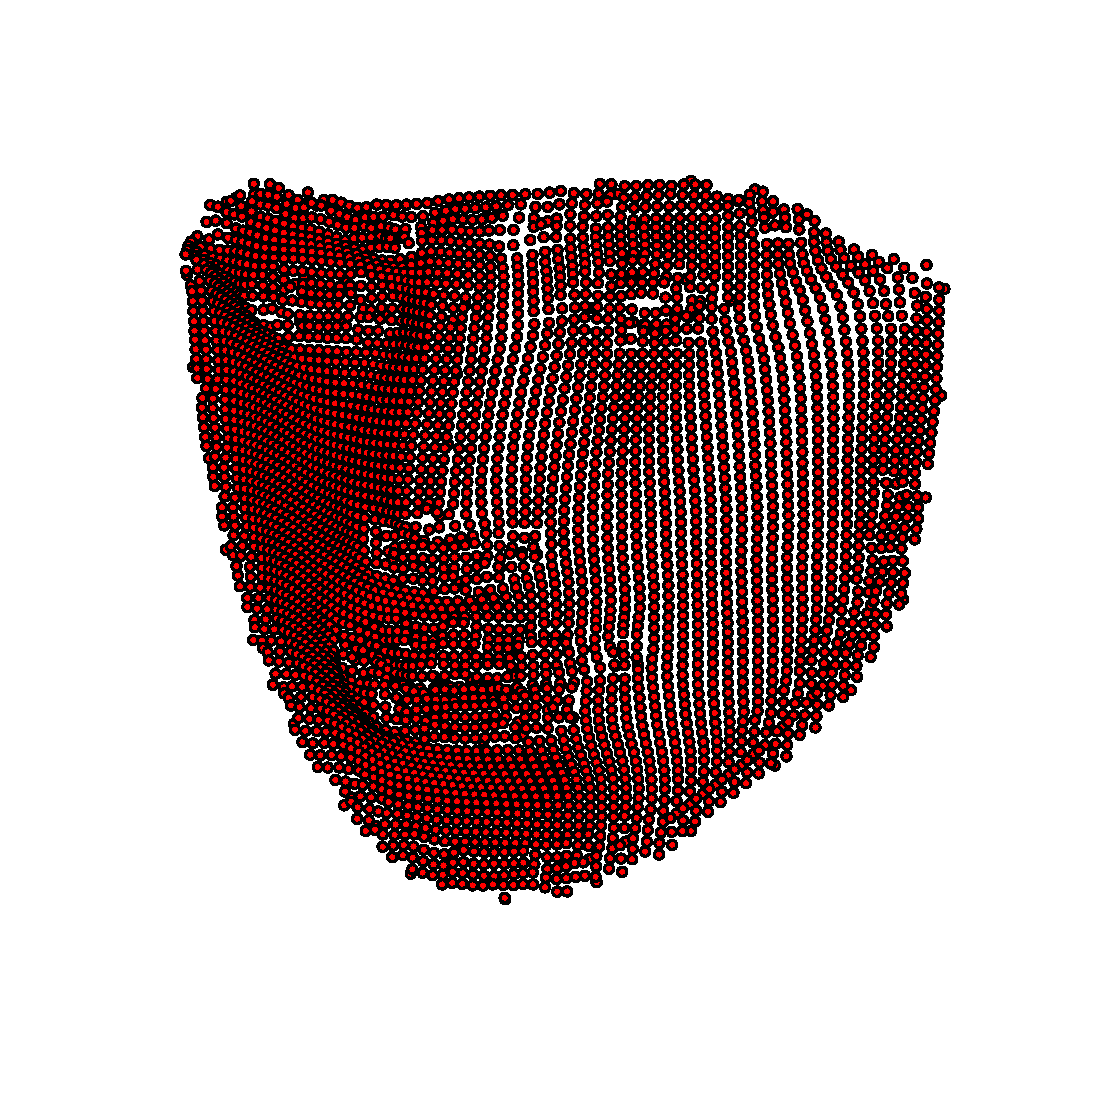
\includegraphics[width=\textwidth]{resources/Fig_dAAM/of_shape}
%     \end{subfigure}
%   	\hfill
%     \begin{subfigure}[b]{0.22\textwidth}
%             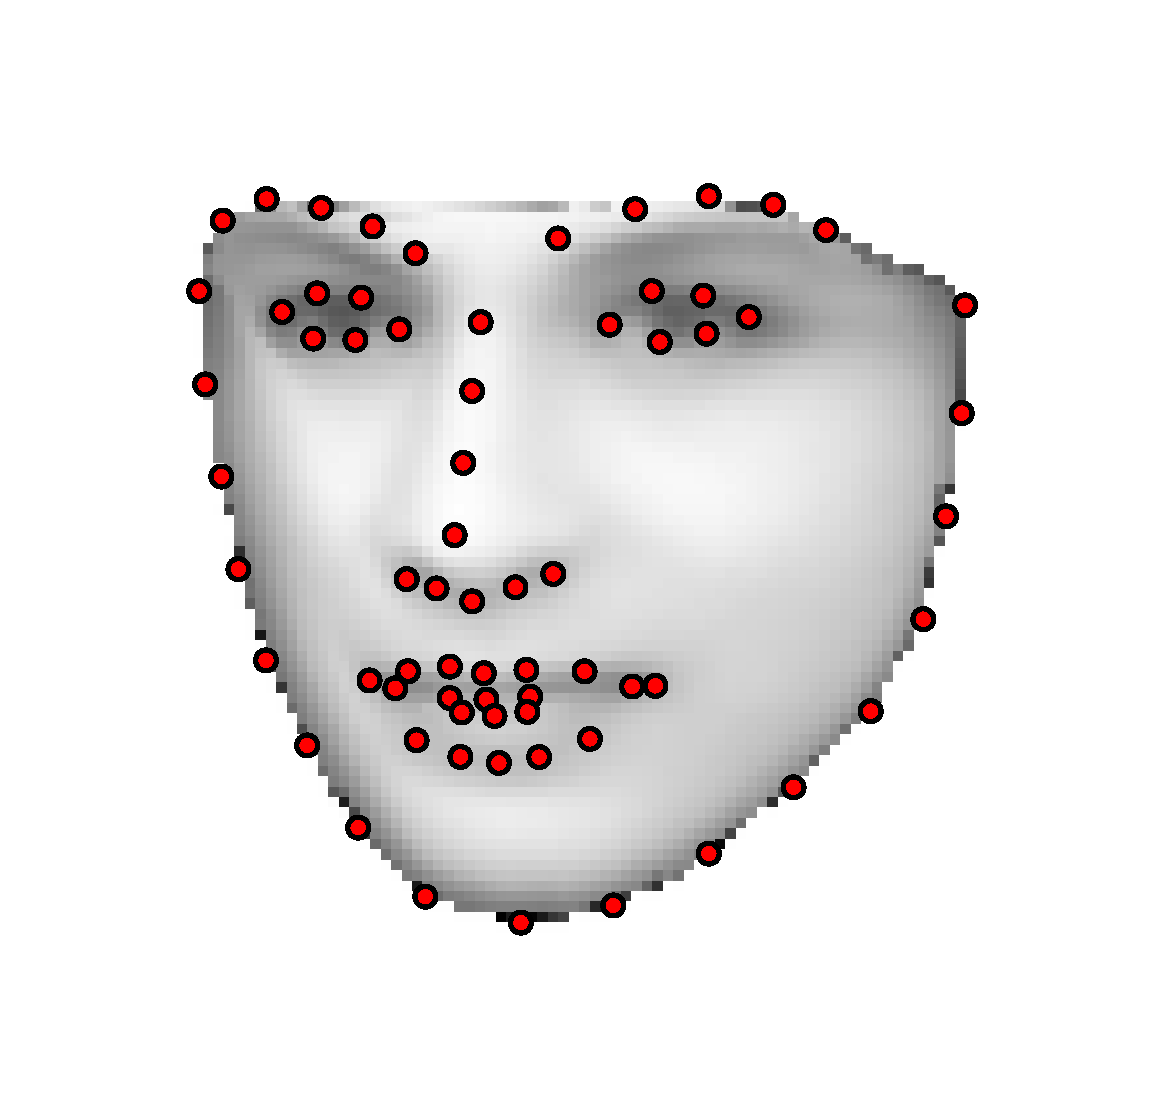
\includegraphics[width=\textwidth]{resources/Fig_dAAM/of_app}
%     \end{subfigure}
%     \caption{Dense Deformable Model}
%     \label{fig:models}
% \end{figure}

% \begin{figure}[h!]
%     \centering
%     \begin{subfigure}[b]{0.22\textwidth}
%             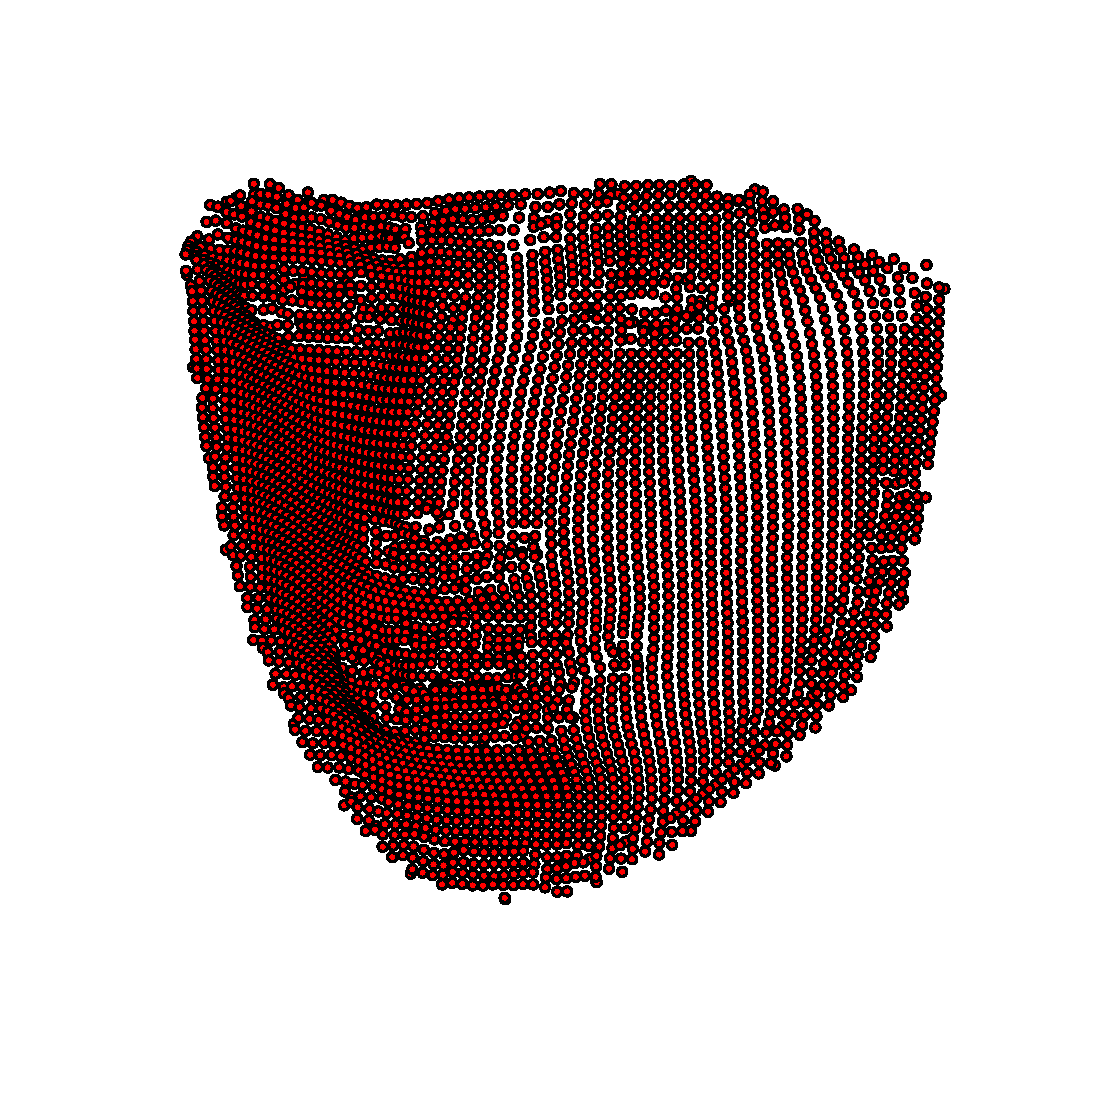
\includegraphics[width=\textwidth]{resources/Fig_dAAM/of_shape}
%     \end{subfigure}
%   	\hfill
%     \begin{subfigure}[b]{0.22\textwidth}
%             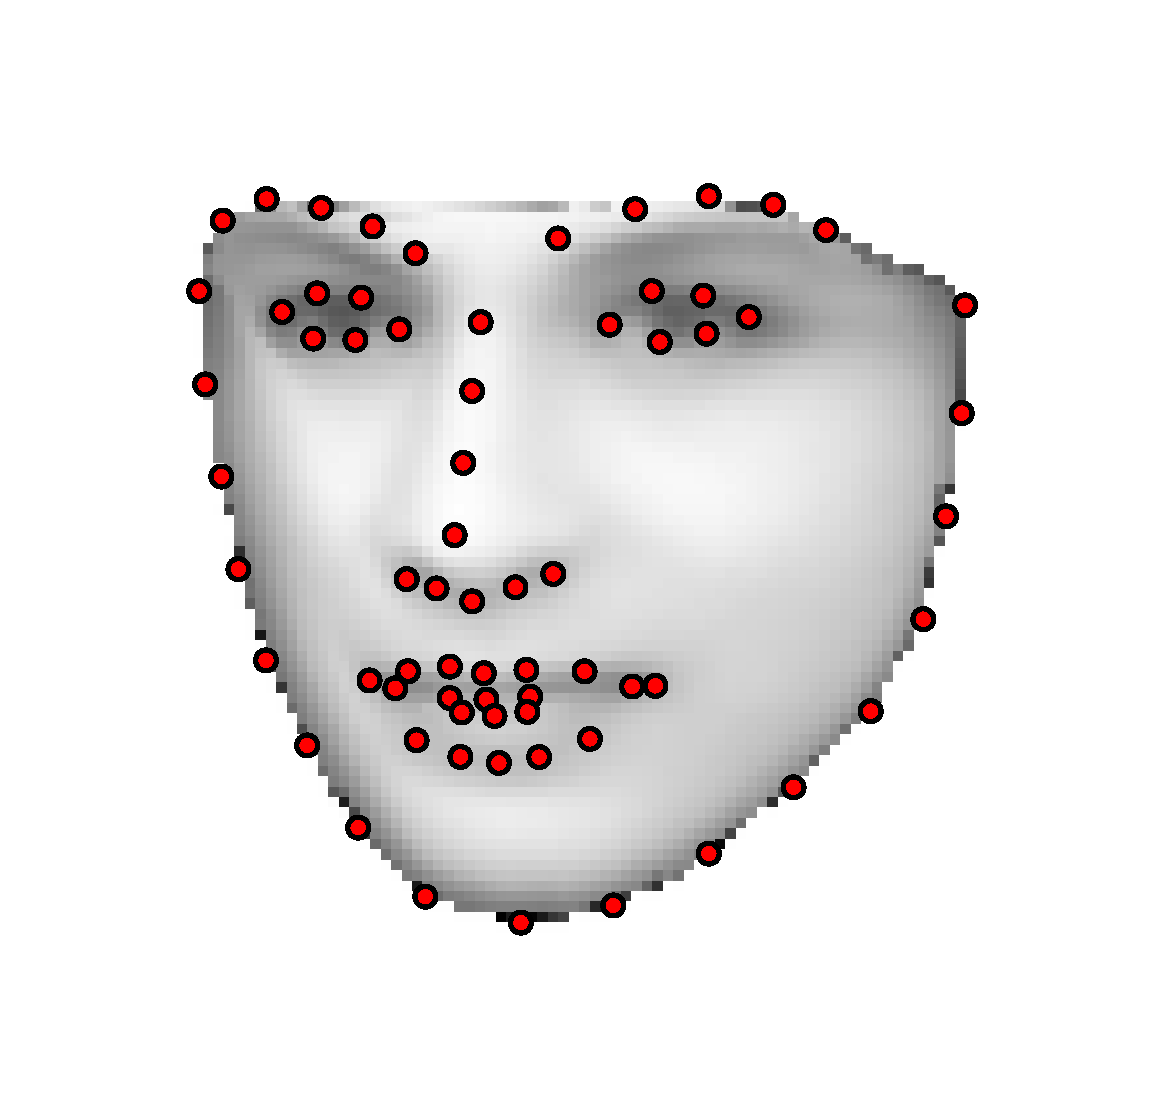
\includegraphics[width=\textwidth]{resources/Fig_dAAM/of_app}
%     \end{subfigure}
%     \caption{Dense Deformable Model}
%     \label{fig:models}
% \end{figure}

\vspace{0.3cm}
{\refstepcounter{steps}\label{sec:step4}\subsection*{Step 4: Dense and Patch-Based Deformable Models}}
% \subsection{Dense and Patch-Based Active Appearance Models}





The deformation fields obtained from Step~\ref{sec:step3} can be used to naturally build two different kinds of effective Active Appearance Models (AAMs) \cite{Cootes2001, Matthews2004}: \emph{dense} \cite{ramnath2008increasing, Amberg2009, anderson2014using} and \emph{patch-based} \cite{Tzimiropoulos2014}. The only difference between these two AAM formulations is on the way that the shape is represented and, thus, the manner in which the texture is sampled. Each one of them is suitable for object classes with specific properties. The dense AAM provides an exceptionally effective modeling and fitting for non-articulated objects, such as ears and faces, whose appearance has characteristic structures that spread all over their region (even if these structures cannot be consistently annotated). On the other hand, there exist other challenging object classes, such as arms and legs, that not only cannot be consistently annotated with landmarks, but their appearance is distinctive only on the object's outline and not in its interior region. Especially in the case of human body parts, they are almost always covered by clothes, which makes it impossible to construct robust texture models.

\paragraph{Dense Active Appearance Model} Since all the deformation fields acquired by Step~\ref{sec:step3} are defined for the pixels of the reference SVS image, the spatial positions $\bm{x}_i=(x_i, y_i)$ of these pixels can be treated as point landmarks and the deformation fields as dense annotations of the object's shape. Consequently, building a dense shape model reduces to normalising these dense annotations with respect to a global similarity transform (typically using Procrustes Analysis) and applying PCA. A shape instance can be generated by the resulting shape model as:
\begin{equation}
    \bm{s}(\bm{p}) = \bm{\bar{s}} + \bm{S} \bm{p}
    \label{eq:shape_model}
\end{equation}
where $\bm{\bar{s}}$ is mean shape, and $\bm{S}$ and $\bm{p}$ are the shape bases and shape parameters, respectively.

By making explicit use of the one-to-one correspondence between pixels on the reference frame and on the deformation fields, the motion model of sparse holistic AAMs \cite{Cootes2001, Matthews2004} (piece-wise affine, thin-plates splines \cite{Bookstein1989}) is replaced by sampling all pixel values onto the reference frame. Let us define this sampling function, given a shape instance $\bm{s}(\bm{p})$, as $\mathcal{W}(\bm{s}(\bm{p}))$. Once the images have been warped, the texture model is obtained by applying PCA on them. A texture instance can be generated as:
\begin{equation}
    \bm{t}(\bm{c}) = \bm{\bar{t}} + \bm{T} \bm{c}
	\label{eq:tex_model}
\end{equation}
where $\bm{t}$ is the mean texture, and $\bm{T}$ and $\bm{c}$ are the texture bases and texture parameters, respectively.

Given a test image $\mathbf{I}$, the fitting process involves the minimization of the following cost function:
\begin{equation}
    \arg\min_{\bm{p}, \bm{c}}\|\bm{I}(\mathcal{W}(\bm{s}(\bm{p}))) - \bm{t}(\bm{c})\|_2^2
	\label{eq:aam_cost}
\end{equation}
This optimization problem is typically solved using the inverse-compositional Gauss-Newton algorithm, for which different variations have been proposed \cite{Matthews2004, Papandreou2008, Amberg2009, Tzimiropoulos2013, Alabort2014}. Note that the existence of the sampling function $\mathcal{W}()$ instead of a non-linear warping function has the advantage that all existing efficient gradient descent algorithms become exact.

\paragraph{Outline Patch-Based Active Appearance Model (PAAM)} The object classes for which the interior appearance does not have specific structure are modeled using patch-based AAMs \cite{Tzimiropoulos2014} trained on a set of sparse landmarks. Especially for human body parts (arms, legs), we strongly believe that the points located to the outline of the object are more suitable compared to the internal ones that correspond to the skeleton joints, which are commonly used by current literature \cite{buehler2011upper,charles2013domain,pfister2015flowing,yang2013articulated}.

The main differences between the patch-based and dense AAMs are that (a)~the densified shape instances are sub-sampled to include only the outline points, and (b)~the texture representation involves the sampling a neighbourhood around each point instead of a single pixel. Specifically, in order to build the outline sparse shape model, we simply select the outline points on the SVS reference frame. Then, by taking advantage of the dense correspondences obtained by Step \ref{sec:step3}, the shape model is trained in a similar way as in the dense case. Moreover, similar to the dense case, the texture model is built by sampling the image values from the sparse shape locations, i.e. $\mathcal{W}(\bm{s}(\bm{p}))$. However, contrary to dense AAMs, we sample a patch that is centred around each landmark point. These patches are then vectorised and concatenated in a single texture vector. Note that the optimization process remains exactly the same.


\section{Experimental Evaluation}

We evaluate the performance of the proposed methodology for the task of human body pose correspondence estimation, as well as non-rigid alignment ``in-the-wild''. For further experimental results, please refer to the supplementary material. Note that all steps of the proposed pipeline were implemented using the Menpo Project~\cite{menpo14}.

%Results of quantitative and qualitative evaluations are reported.

\begin{figure}[t!]
    \centering
    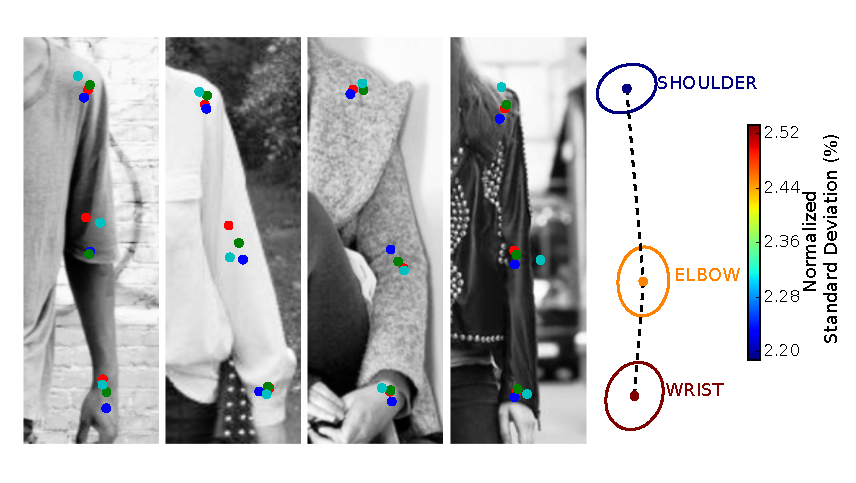
\includegraphics[width=\columnwidth]{resources/Fig_Variance/final}
    \caption{Example of human pose annotation for left arm among 4 annotators. The large variance highlights the difficulty of obtaining consistent landmarks.}
    \label{fig:variance}
\end{figure}

\begin{figure*}[!t]
    \newcommand{\fh}{0.24\columnwidth}
    \centering
    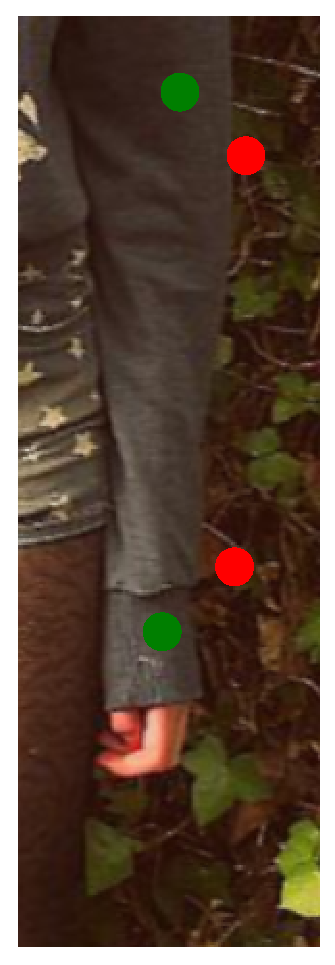
\includegraphics[height=\fh]{resources/Fixing/fix_1}
    \hfill
    \includegraphics[height=\fh]{resources/Fixing/fix_2}
    \hfill
    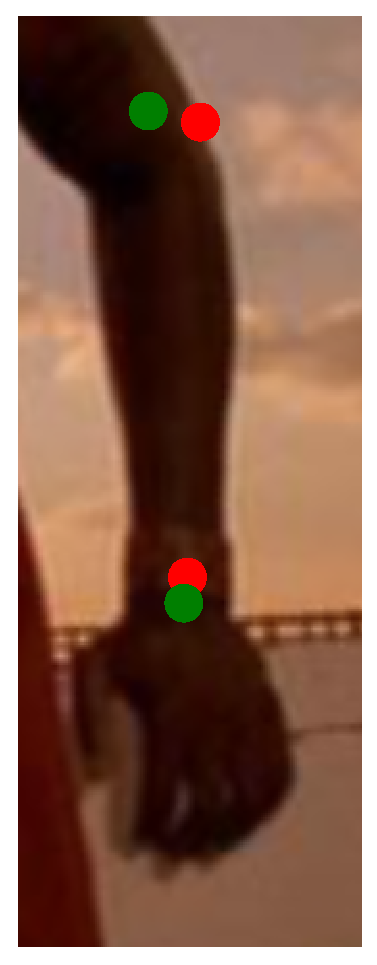
\includegraphics[height=\fh]{resources/Fixing/fix_3}
    \hfill
    \includegraphics[height=\fh]{resources/Fixing/fix_5}
    \hfill
    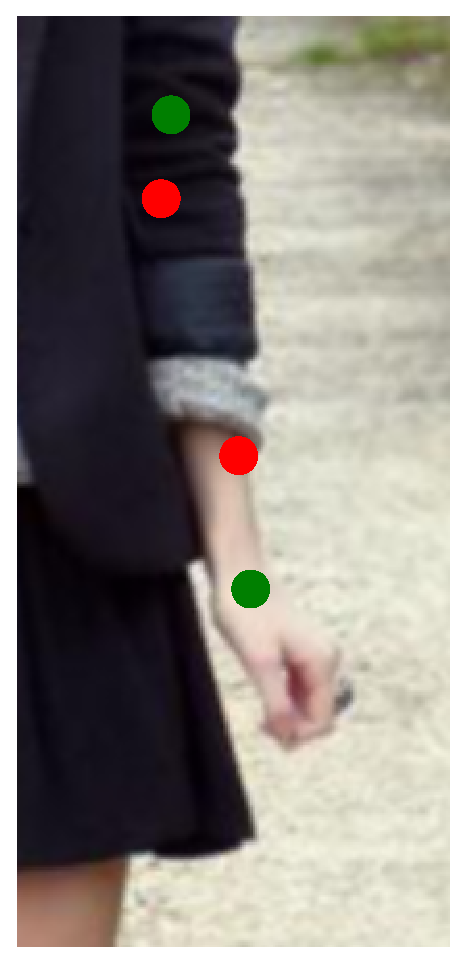
\includegraphics[height=\fh]{resources/Fixing/fix_6}
    \hfill
    \includegraphics[height=\fh]{resources/Fixing/fix_7}
    \hfill
    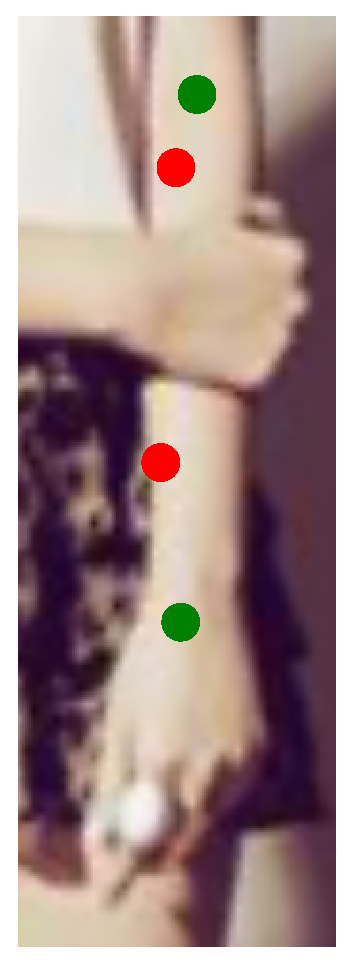
\includegraphics[height=\fh]{resources/Fixing/fix_8}
    \hfill
    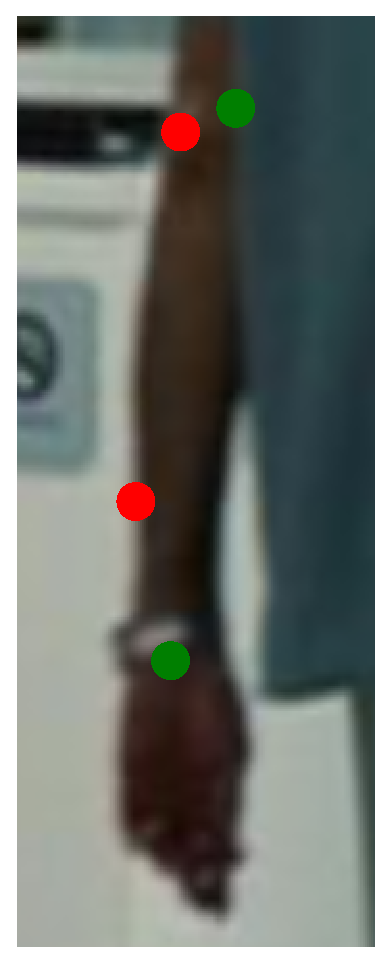
\includegraphics[height=\fh]{resources/Fixing/fix_9}
    \hfill
    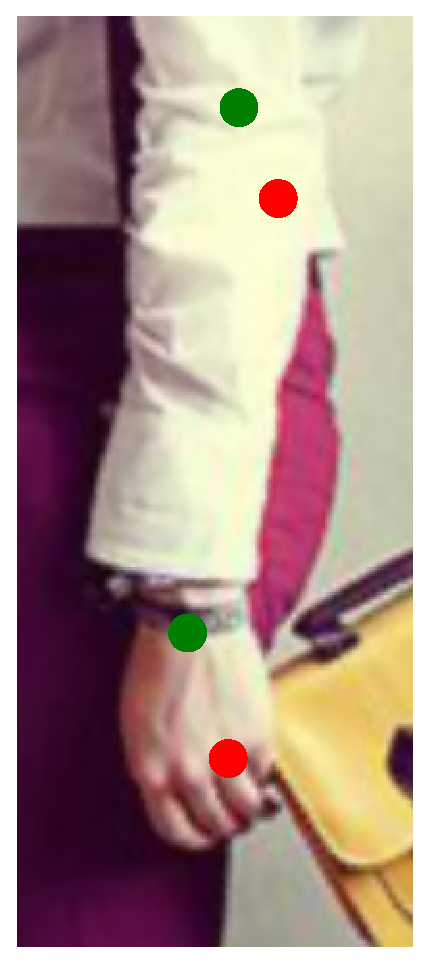
\includegraphics[height=\fh]{resources/Fixing/fix_10}
    \hfill
    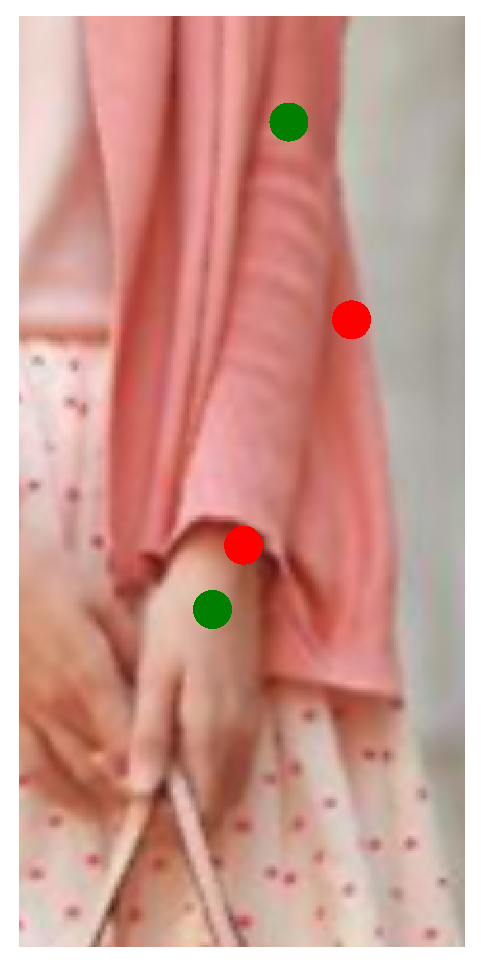
\includegraphics[height=\fh]{resources/Fixing/fix_20}
    \hfill
    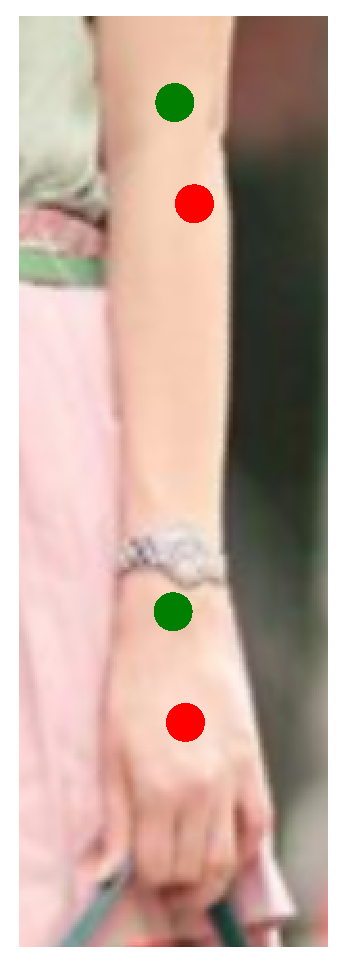
\includegraphics[height=\fh]{resources/Fixing/fix_12}
    \hfill
    \includegraphics[height=\fh]{resources/Fixing/fix_13}
    \hfill
    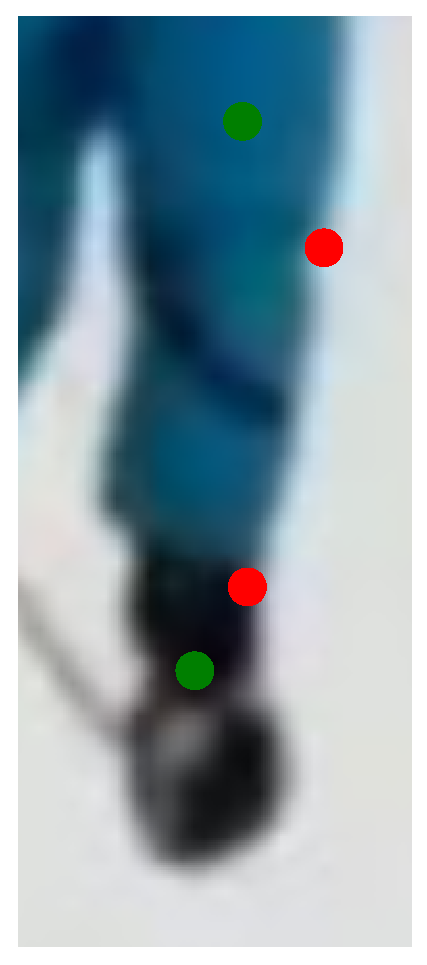
\includegraphics[height=\fh]{resources/Fixing/fix_14}
    \hfill
    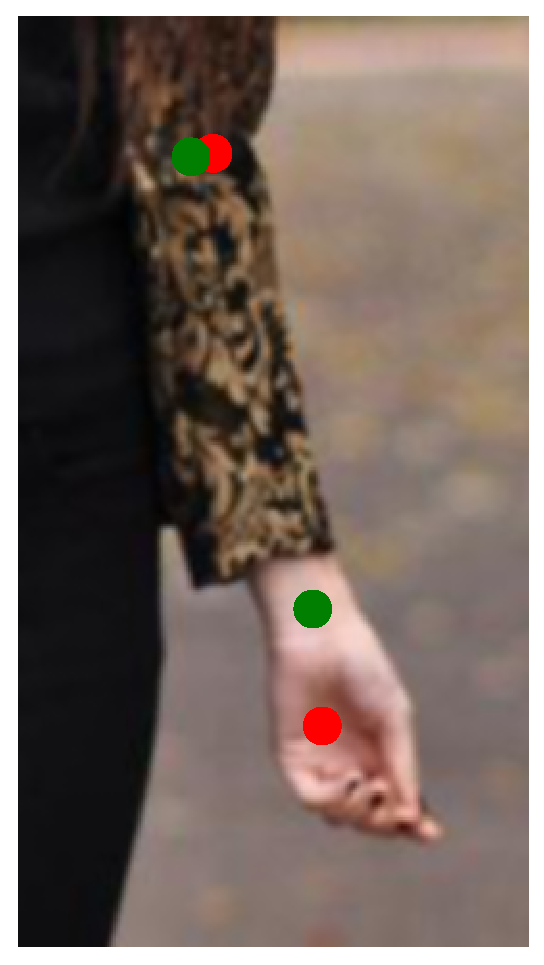
\includegraphics[height=\fh]{resources/Fixing/fix_15}
    \hfill
    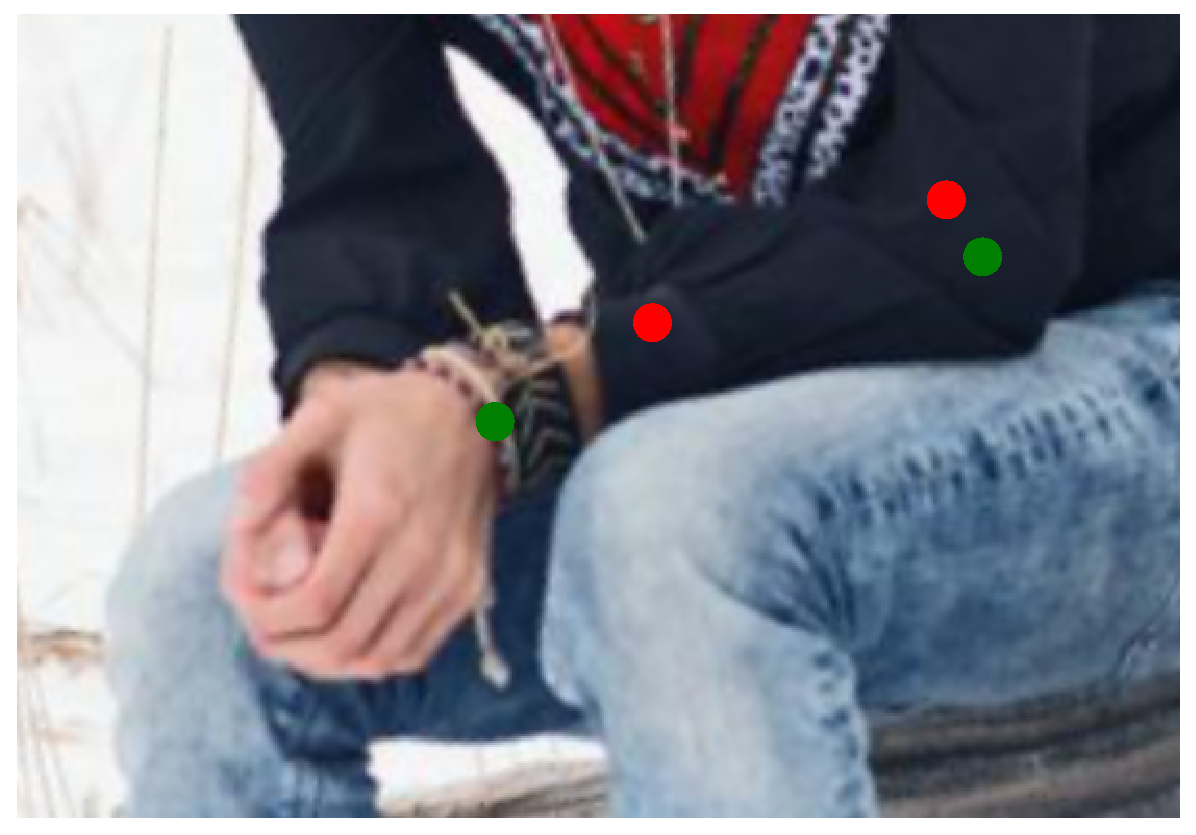
\includegraphics[height=\fh]{resources/Fixing/fix_17}
    \hfill
    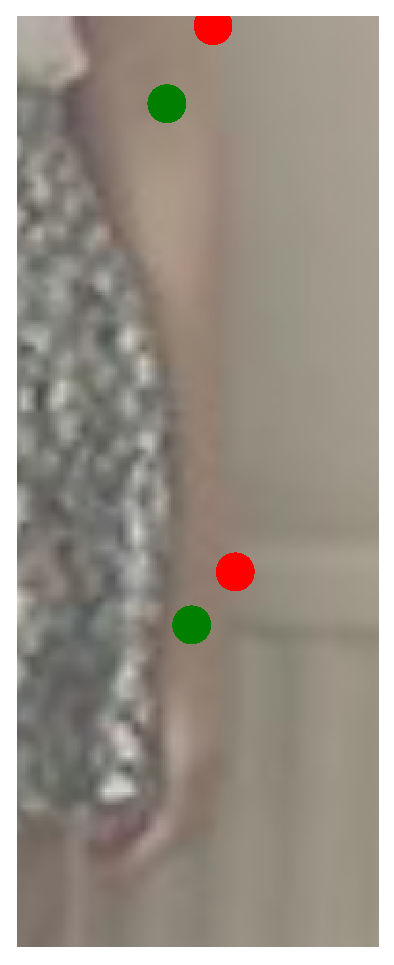
\includegraphics[height=\fh]{resources/Fixing/fix_18}
    \caption{Demonstration of annotation correction using our method for the experiment of Section \ref{exp:qualitative}. \emph{Red} dots refer to officially provided landmarks, and \emph{green} dots are corrected position.}
    \label{fig:qualitative}
\end{figure*}

\begin{figure*}[!t]
    \newcommand{\ofh}{0.24\columnwidth}
    \centering
    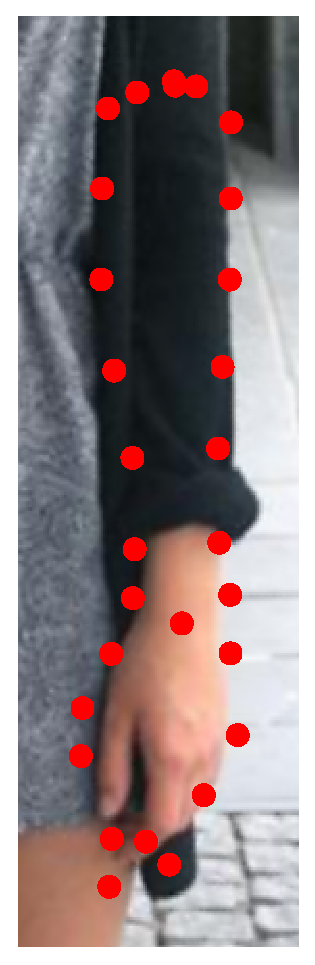
\includegraphics[height=\ofh]{resources/Fittings/20.eps}
    \hfill
    \includegraphics[height=\ofh]{resources/Fittings/3.eps}
    \hfill
    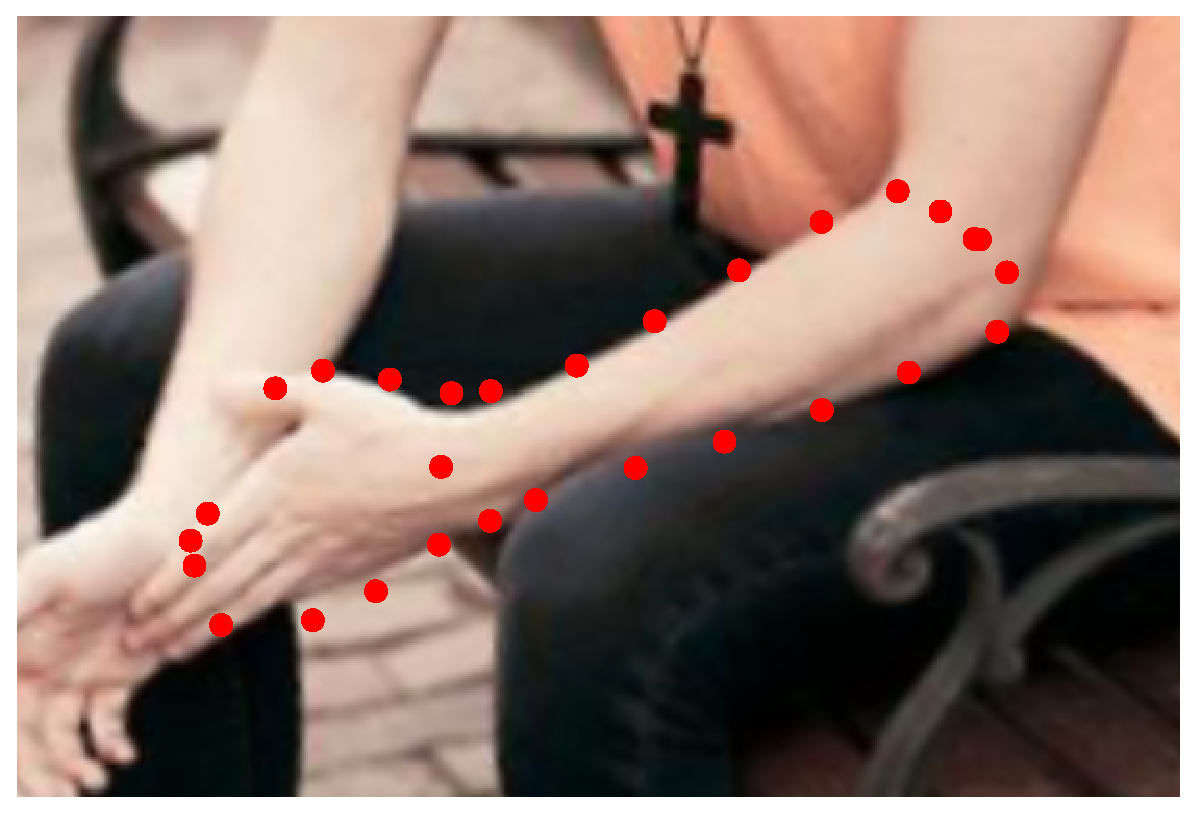
\includegraphics[height=\ofh]{resources/Fittings/19.eps}
    \hfill
    \includegraphics[height=\ofh]{resources/Fittings/4.eps}
    \hfill
    \includegraphics[height=\ofh]{resources/Fittings/6.eps}
    \hfill
    \includegraphics[height=\ofh]{resources/Fittings/15.eps}
    \hfill
    \includegraphics[height=\ofh]{resources/Fittings/7.eps}
    \hfill
    \includegraphics[height=\ofh]{resources/Fittings/8.eps}
    \hfill
    \includegraphics[height=\ofh]{resources/Fittings/13.eps}
    \hfill
    \includegraphics[height=\ofh]{resources/Fittings/17.eps}
    \\
    \includegraphics[height=\ofh]{resources/Fittings/21.eps}
    \hfill
    \includegraphics[height=\ofh]{resources/Fittings/23.eps}
    \hfill
    \includegraphics[height=\ofh]{resources/Fittings/25.eps}
    \hfill
    \includegraphics[height=\ofh]{resources/Fittings/27.eps}
    \hfill
    \includegraphics[height=\ofh]{resources/Fittings/29.eps}
    \hfill
    \includegraphics[height=\ofh]{resources/Fittings/31.eps}
    \hfill
    \includegraphics[height=\ofh]{resources/Fittings/33.eps}
    \hfill
    \includegraphics[height=\ofh]{resources/Fittings/35.eps}
    \hfill
    \includegraphics[height=\ofh]{resources/Fittings/36.eps}
    \hfill
    \includegraphics[height=\ofh]{resources/Fittings/37.eps}
    \hfill
    \includegraphics[height=\ofh]{resources/Fittings/38.eps}
    \hfill
    \includegraphics[height=\ofh]{resources/Fittings/39.eps}
    \caption{Demonstration of outline fitting of patch-based AAM on arms.}
    \label{fig:outline_fitting}
    \vspace{-5pt}
\end{figure*}




\subsection{Non-rigid Object Alignment In-the-Wild}
\label{exp:daam_benchmark}
Herein, we compare the fitting accuracy of the dAAMs that are trained with our proposed framework with holistic sparse AAMs~\cite{Cootes2001,Matthews2004,antonakos2015feature}. We consider two object classes that demonstrate rich texture: face and ear.

\noindent\textbf{Databases \& Error Metrics} In the case of face, we trained both models using the 811 training images of the Labelled Faces Parts in-the-Wild (LFPW)~\cite{belhumeur2013localizing}. Sparse AAMs were built from the 68 points annotations provided by~\cite{sagonas_iccv_300w_2013,sagonas2016faces}. Our dAAMs were built as described in Step~\ref{sec:step4}. In both cases, the appearance is represented using pixel intensities. The results are reported on the 224 images of the LFPW testset. The fitting error is evaluated as the point-to-point distance normalised by the face's size, as proposed in~\cite{Zhu2012}.

In the case of human ear, given the lack of publicly available annotated databases, we collected 605 high resolution images captured under unconstrained conditions from online search engines. The images were manually annotated with respect to 55 sparse landmarks, as well as the curve annotations proposed in this paper. Examples of these two types of annotations are shown in Figure~\ref{fig:intro}. We randomly split the database into two disjoint sets of training (500) and testing (105) images. The training and evaluation of the two models is done in the same way as in the case of face.

\begin{figure}[b!]
    \vspace{-5pt}
    \centering
    \includegraphics[width=0.6\columnwidth]{resources/DAAMBenchmark/legend}
    \\
    \includegraphics[width=0.48\columnwidth]{resources/DAAMBenchmark/face}
    \includegraphics[width=0.48\columnwidth]{resources/DAAMBenchmark/ear}
    \caption{CEDs of faces and ears fitting performance for the experiment of Section \ref{exp:daam_benchmark}.}
    \label{fig:daam_benchmark}
\end{figure}

\noindent\textbf{Results} We report the results in Figure~\ref{fig:daam_benchmark} using Cumulative Error Distribution (CED) curves. By visual inspection of the results, we determined that the fitting is adequately accurate for errors less than 0.1 and 0.06 for the ear and face, respectively. The results indicate that dAAMs marginally outperform sparse AAMs. Therefore, the proposed pipeline is capable of dealing with the complex structure of non-rigid shapes and train dAAMs from simple curve line annotations which can compete and even outperform the commonly-used sparse AAMs trained on carefully annotated images.


\subsection{Arm Pose Estimation}
\label{exp:benchmark}
In this experiment, we aim to compare the effect of training a deformable model of human arm using: (i)~our proposed outline sparse landmarks, and (ii)~the standard skeleton joints annotations that are commonly employed in literature. For this purpose, we employ the patch-based AAM as described in Step~\ref{sec:step4}. Additionally, we compare our methodology with the current state-of-the-art.


\begin{figure}[b!]
    \vspace{-5pt}
    \centering
    \includegraphics[width=\columnwidth]{resources/HandBenchmark/legend}
    \\
    \includegraphics[width=0.48\columnwidth]{resources/HandBenchmark/wrist}
    \includegraphics[width=0.48\columnwidth]{resources/HandBenchmark/elbow}
    \caption{CEDs over skeleton landmarks on BBC Pose database for the experiment of Section  \ref{exp:benchmark}.}
    \label{fig:hand_benchmark}
\end{figure}


\noindent\textbf{Dataset \& Error Metric} We opted to report quantitative results on the BBC Pose database~\cite{pfister2015flowing}, which provides the most consistent and accurate joints annotations compared to the rest of existing databases. The training of the outline patch-based AAM was performed after obtaining 29 outline landmarks using our proposed framework. We used 891 training images from a combination of datasets, including H3D~\cite{PoseletsICCV09}, Microsoft COCO~\cite{lin2014microsoft}, MPII~\cite{andriluka14cvpr}, Fashion Pose~\cite{dantone2013human}, FLIC~\cite{sapp2013modec} and BBC Pose~\cite{pfister2015flowing}. SIFT features~\cite{PoseletsICCV09} are adopted for the image representation in our model. The fitting procedure on the BBC Pose database is initialised using a simplistic in-house deep convolutional neural network.

In order to compare with current state-of-the-art on BBC Pose, we used the same error metric as the one in~\cite{pfister2015flowing}, which normalises testing images in order to have a height of 256 pixels. Once again, the performance is visualised using CED curves. The results for this experiment are reported on 1000 testing images from BBC Pose, which utilises 7 skeleton landmarks to annotate the human upper-body pose. Note that in the case of our model, the final joints locations required for evaluation are retrieved from the dense correspondence acquired with our proposed method. On the contrary, the rest of the methods are trained on this 7-points mark-up, thus directly return their estimated locations.

\noindent\textbf{Results} Figure~\ref{fig:hand_benchmark} reports the results of our model trained on the outline landmarks (Outline PAAM), as well as the current state-of-the-art techniques which include: Buehler~\cite{buehler2011upper}, Charles14~\cite{charles2014upper}, Charles13~\cite{charles2013domain}, Pfister14~\cite{pfister2015deep}, Ramanan~\cite{yang2013articulated} and Pfister15~\cite{pfister2015flowing}. As can be seen, our outline part-based AAM model outperforms the state-of-the-art for this task, even though it is not trained directly on the wrist and elbow points, thus it is not tailored for locating them. In particular, our model outperforms the currently best method~\cite{pfister2015flowing} by a notable amount (9\% with error less than 6pt) on wrist, as well as marginal improvement on elbow estimation. Figure~\ref{fig:outline_fitting} shows some indicative qualitative fitting results.

In the same experiment we prove that it is more advantageous to train a deformable model using the outline landmarks rather than the skeleton points. This is done by building a patch-based AAM on the same training data and with identical settings using both annotation schemes. As it can be seen from the  CED curves of Figure~\ref{fig:hand_benchmark}, our model trained on outline landmarks (Outline PAAM) notable outperforms the skeleton-based model for both wrist and elbow. We believe that this is a remarkable result, which indicates that out proposed outline mark-up can lead to a significant improvement of current state-of-the-art techniques.


% \begin{figure*}[!t]
%     \newcommand{\fh}{0.24\columnwidth}
%     \centering
%     \includegraphics[height=\fh]{resources/Fixing/fix_1}
%     \includegraphics[height=\fh]{resources/Fixing/fix_2}
%     \includegraphics[height=\fh]{resources/Fixing/fix_3}
%     \includegraphics[height=\fh]{resources/Fixing/fix_5}
%     \includegraphics[height=\fh]{resources/Fixing/fix_6}
%     \includegraphics[height=\fh]{resources/Fixing/fix_7}
%     \includegraphics[height=\fh]{resources/Fixing/fix_8}
%     \includegraphics[height=\fh]{resources/Fixing/fix_9}
%     \includegraphics[height=\fh]{resources/Fixing/fix_10}
%     \includegraphics[height=\fh]{resources/Fixing/fix_20}
%     \includegraphics[height=\fh]{resources/Fixing/fix_12}
%     \includegraphics[height=\fh]{resources/Fixing/fix_13}
%     \includegraphics[height=\fh]{resources/Fixing/fix_14}
%     \includegraphics[height=\fh]{resources/Fixing/fix_15}
%     \includegraphics[height=\fh]{resources/Fixing/fix_17}
%     \includegraphics[height=\fh]{resources/Fixing/fix_18}
%     \caption{Demonstration of annotation correction using our method for experiment \ref{exp:qualitative}. \emph{Red} dots refer to officially provided landmarks, and \emph{green} dots are corrected position.}
%     \label{fig:qualitative}
% \end{figure*}

% \begin{figure*}[!t]
%     \newcommand{\ofh}{0.24\columnwidth}
%     \centering
%     \includegraphics[height=\ofh]{resources/Fittings/20.eps}
%     \includegraphics[height=\ofh]{resources/Fittings/3.eps}
%     \includegraphics[height=\ofh]{resources/Fittings/19.eps}
%     \includegraphics[height=\ofh]{resources/Fittings/4.eps}
%     \includegraphics[height=\ofh]{resources/Fittings/6.eps}
%     \includegraphics[height=\ofh]{resources/Fittings/15.eps}
%     \includegraphics[height=\ofh]{resources/Fittings/7.eps}
%     \includegraphics[height=\ofh]{resources/Fittings/8.eps}
%     \includegraphics[height=\ofh]{resources/Fittings/13.eps}
%     \includegraphics[height=\ofh]{resources/Fittings/17.eps}
%     \\
%     \includegraphics[height=\ofh]{resources/Fittings/21.eps}
%     \includegraphics[height=\ofh]{resources/Fittings/23.eps}
%     \includegraphics[height=\ofh]{resources/Fittings/25.eps}
%     \includegraphics[height=\ofh]{resources/Fittings/27.eps}
%     \includegraphics[height=\ofh]{resources/Fittings/29.eps}
%     \includegraphics[height=\ofh]{resources/Fittings/31.eps}
%     \includegraphics[height=\ofh]{resources/Fittings/33.eps}
%     \includegraphics[height=\ofh]{resources/Fittings/35.eps}
%     \includegraphics[height=\ofh]{resources/Fittings/36.eps}
%     \includegraphics[height=\ofh]{resources/Fittings/37.eps}
%     \includegraphics[height=\ofh]{resources/Fittings/38.eps}
%     \includegraphics[height=\ofh]{resources/Fittings/39.eps}
%     \caption{Demonstration of outline fitting of patch-based AAM on arms.}
%     \label{fig:outline_fitting}
% \end{figure*}

\subsection{Annotation Correction}
\label{exp:qualitative}
The final experiment demonstrates that it is feasible to use the proposed arm model in order to correct the annotations provided by current datasets. As mentioned above there are inconsistencies in the annotations of MPII~\cite{andriluka14cvpr}, Fashion Pose~\cite{dantone2013human} and FLIC~\cite{sapp2013modec}. Due to the large variance in arm pose, it is difficult even for trained annotators to obtain consistent annotations between them. As proof of concept, Figure~\ref{fig:variance} reports the standard deviation observed between the annotations of 4 trained humans that were requested to annotate 120 images of left arms from Fashion Pose~\cite{dantone2013human} with respect to the shoulder, elbow and wrist.

By applying our outline patch-based AAM on the aforementioned databases, we managed to greatly correct the currently available annotations of the arm. Figure~\ref{fig:qualitative} shows indicative examples of the corrected landmarks. There is no doubt that points after correction demonstrate more consistency among images. We make the corrected annotations publicly available\textsuperscript{\ref{foot:annotations}}.


















% \begin{table}[b!]
%     \small
%     \centering
%     \begin{tabular}{|l|c|c|c||c|c|c|}
%         \hline
%                             & \multicolumn{3}{c||}{Wrist} & \multicolumn{3}{c|}{Elbow}\\
%         \hline
%         \emph{Method}       & \emph{mean} & \emph{std} & $\leq 6pt$ & \emph{mean} & \emph{std} & $\leq 6pt$\\
%         \hline\hline
%         Buehler             & 12.08    & 19.94        & 44.5\%       & 12.94    & 14.65        & 34.4\%\\
%         Charles14           & 11.81    & 20.89        & 54.2\%       &  8.30    & 11.00        & \textbf{55.2\%}\\
%         Charles13           & 13.78    & 22.39        & 43.3\%       & 13.17    & 18.74        & 46.3\%\\
%         Pfister14           & 14.69    & 17.89        & 29.7\%       & 14.60    & 10.59        & 14.0\%\\
%         Ramanan             & 15.59    & 19.04        & 22.6\%       & 15.53    & 10.82        & 15.8\%\\
%         Pfister15           & 7.62     & 11.04        & 54.1\%       &  8.84    & 11.44        & 54.9\%\\
%         \hline\hline
%         Ours                & \textbf{6.71}& \textbf{10.90}   & \textbf{63.1\%}       & \textbf{8.20}     &  \textbf{10.54}        & 52.1\%\\
%         \hline
%     \end{tabular}
%     \caption{Fitting statistics on BBC Pose database for experiment \ref{exp:benchmark}}
%     \label{tab:hand_benchmark}



\section{Conclusion}
Learning and fitting statistical deformable models (SDMs) is one of the most important areas in computer vision. Generally, in order to train a SDM, a set of predefined correspondences are required. In some objects, such as human face, semantically meaningful correspondences can be found, but require laborious manual annotations; on other objects it is very difficult, or even impossible. In this paper, we propose one of the first comprehensive procedures for establishing correspondences (that do not necessarily correspond to semantically meaningful object landmarks) in arbitrary objects with minimal amount of human annotation. We apply the proposed approach for the construction of the first, to the best of our knowledge, highly-descriptive SDM for the human arm. 

\section{Supplementary}
\begin{figure*}[!b]
\centering
\includegraphics[width=\textwidth]{resources/Suplementory_Meterial/Models/models}
\caption{Principal components of dAAMs built on ears (top) and faces (bottom). The mean (middle columns) as well as the first five principal components are visualised for both shape (left) and appearance (right). $\pm 3$ times the variance of the corresponding component is used in each case.}
\label{fig:pcamodel}
\end{figure*}


%%%%%%%%% Appendix
\section*{Introduction}
In this supplementary material, we provide additional algorithmic details for our shape flow estimation, as well as additional visualisations and evaluations for the dense and patch-based AAMs that were constructed using the proposed framework.


\appendix
\section{Implementation of Shape Flow Estimation}
\label{sec:cost_function}


As mentioned in the main paper (Section 3, Step 3), we propose to estimate the shape flow by minimising the following energy:
\vspace{-5pt}
\begin{align}
E_{sf} & =\alpha
\int_{\Omega}\sum_{n=1}^{N_t} \|\bm{d}(\bx+\bm{u}_n(x);n)-\bm{d}(x;0)\| \ud \bx \label{eq:costfunc}\\
    &+ \beta \int_{\Omega}\sum_{n=1}^{N_t}\|\bm{u}_n(\bx)-\sum_{i=1}^R\bm{q}_i(n)\bm{v}_i(\bx)\|^2 \ud \bx \label{eq:lowrank}\\
    &+
\int_\Omega  \sum_{i=1}^R \,\, \left \|    \nabla \bm{v}_i(\bx)    \right \|  \,\ud \bx \label{eq:TVterm}
\vspace{-5pt}
\end{align}
We minimise this energy jointly with respect to $\bm{u}_n(\bx)$ and $\bm{v}_i(\bx)$, which correspond to the
two sets of unknown shape flows.
We implement this minimisation based on the optimisation algorithm described in \cite{Garg:2013hu} and the relevant publicly available code \footnote{https://bitbucket.org/troussos/mfsf/downloads}.
However, we modify this algorithm so that, instead of initialising the coarse-to-fine and warping iterations with a zero flow, we use Thin Plate Splines (TPS) \cite{Bookstein1989} interpolation of the initial correspondence vectors described in Section 3, Step 2 of the main paper.
This yields a significantly better initial location of the highly-nonconvex objective function and improves the computational efficiency, since much less coarse-to-fine pyramids are needed.

Note that in every coarse-to-fine and warping iteration, we use an initialisation that comes from the previous iteration. We approximate the data term \eqref{eq:costfunc} by linearising the SVS images $\bm{d}(\bx;n)$ around the initialisation. After that, the energy becomes convex and we optimise it by employing alternating optimisation with respect to $\bm{v}_i(\bx)$ and $\bm{u}_n(\bx)$. The minimisation with respect to $\bm{v}_i(\bx)$ is decoupled for every coefficient $i$ and corresponds to Rudin-Osher-Fatemi Total Variation denoising~\cite{rudin92}, which we solve efficiently by applying the first order primal-dual algorithm of~\cite{Chambolle:Pock:JMIV2011}. The minimisation with respect to $\bm{u}_n(x)$ is decoupled for every pixel $\bx$ and every shape index $i$. This minimisation is also implemented by applying the efficient primal-dual algorithm of~\cite{Chambolle:Pock:JMIV2011}.

\section{Dense Active Appearance Models}
\label{sec:daam}

In this section, we report additional qualitative and quantitative evaluations for the Dense Active Appearance Models (dAAMs) of faces and ears that were constructed using the proposed framework.



\subsection{Principal Components and Compactness}



Figure~\ref{fig:pcamodel} visualises the first five shape and appearance principal components of ear and face dAAMs. We observe that in both ear and face cases, the variation of both shape and appearance captured by the model seem plausible.


Figure~\ref{fig:compact} plots the variance ration of the face dAAM, which provides an indication of the compactness of the model. The compactness is compared with the one of a standard sparse AAM built on the same data. Note that these are the two shape models that are compared in Figure 9-left of the main paper. We observe that our dAAM is significantly more compact than the sparse AAM, since for any given number of components, it manages to explain a larger portion of the corresponding total variance of the training set. 


\begin{figure}[!t]
    \centering
    \includegraphics[width=\columnwidth]{resources/Suplementory_Meterial/Model_Analysis/cumu_var_ratio}
    \caption{Compactness plots of dAAM (blue) and sparse AAM (red) models for faces. Portion of the corresponding total variance explained as a function of the number of retained principal components.}
    \label{fig:compact}
\end{figure}

\subsection{Dense Shape Reconstruction Ability}

\begin{figure}[!t]
    \centering
    % \vspace*{-0.1in}
    \begin{subfigure}[b]{\columnwidth}
            \includegraphics[width=\textwidth,trim={0 0 0 25pt},clip]{resources/Suplementory_Meterial/Model_Analysis/sr_ear}
        %\caption{dAAMs dense shape reconstruction}
    \end{subfigure}
    \\
    \begin{subfigure}[b]{\columnwidth}
            \includegraphics[width=\textwidth,trim={0 0 0 25pt},clip]{resources/Suplementory_Meterial/Model_Analysis/sr_face}
        %\caption{AAMs dense shape reconstruction}
    \end{subfigure}
    \caption{Dense shape reconstruction errors for ears (top) and faces (bottom), using AAMs (red) and dAAMs (blue). The average normalized dense point-to-point distance error is plotted as a function of the number of principal components of the model.}
    \label{fig:rc_face}
\end{figure}

Figure \ref{fig:rc_face} evaluates the dense shape reconstruction ability of the proposed dAAMs and compares it with that of standard sparse AAMs. Specifically, we use shapes with dense ground-truth annotations and reconstruct them with both AAMs and dAAMs, by projecting on the corresponding model subspace. In the case of AAMs, which only contain a sparse shape model, we densify it using a piecewise affine transformation, which is typically for texture warping of these models. We observe that dAAMs significantly outperform classic AAMs, in terms of dense shape reconstruction accuracy.



\begin{figure*}[!t]
    \newcommand{\ofh}{0.24\columnwidth}
    \centering
    \includegraphics[height=\ofh]{resources/Suplementory_Meterial/ExFit/0001.eps}
    \hfill
    \includegraphics[height=\ofh]{resources/Suplementory_Meterial/ExFit/0002.eps}
    \hfill
    \includegraphics[height=\ofh]{resources/Suplementory_Meterial/ExFit/0003.eps}
    \hfill
    \includegraphics[height=\ofh]{resources/Suplementory_Meterial/ExFit/0004.eps}
    \hfill
    \includegraphics[height=\ofh]{resources/Suplementory_Meterial/ExFit/0005.eps}
    \hfill
    \includegraphics[height=\ofh]{resources/Suplementory_Meterial/ExFit/0006.eps}
    \hfill
    \includegraphics[height=\ofh]{resources/Suplementory_Meterial/ExFit/0007.eps}
    \hfill
    \includegraphics[height=\ofh]{resources/Suplementory_Meterial/ExFit/0008.eps}
    \hfill
    \includegraphics[height=\ofh]{resources/Suplementory_Meterial/ExFit/0009.eps}
    \hfill
    \includegraphics[height=\ofh]{resources/Suplementory_Meterial/ExFit/0010.eps}
    \hfill
    \includegraphics[height=\ofh]{resources/Suplementory_Meterial/ExFit/0011.eps}
    \hfill
    \includegraphics[height=\ofh]{resources/Suplementory_Meterial/ExFit/0012.eps}
    \hfill
    \includegraphics[height=\ofh]{resources/Suplementory_Meterial/ExFit/0013.eps}
    \hfill
    \includegraphics[height=\ofh]{resources/Suplementory_Meterial/ExFit/0014.eps}
    \hfill
    \includegraphics[height=\ofh]{resources/Suplementory_Meterial/ExFit/0015.eps}
    \hfill
    \includegraphics[height=\ofh]{resources/Suplementory_Meterial/ExFit/0017.eps}
    \hfill
    \includegraphics[height=\ofh]{resources/Suplementory_Meterial/ExFit/0018.eps}
    \hfill
    \includegraphics[height=\ofh]{resources/Suplementory_Meterial/ExFit/0019.eps}
    \hfill
    \includegraphics[height=\ofh]{resources/Suplementory_Meterial/ExFit/0020.eps}
    \hfill
    \includegraphics[height=\ofh]{resources/Suplementory_Meterial/ExFit/0021.eps}
    \hfill
    \includegraphics[height=\ofh]{resources/Suplementory_Meterial/ExFit/0022.eps}
    \hfill
    \includegraphics[height=\ofh]{resources/Suplementory_Meterial/ExFit/0023.eps}
    \hfill
    \includegraphics[height=\ofh]{resources/Suplementory_Meterial/ExFit/0024.eps}
    \hfill
    \includegraphics[height=\ofh]{resources/Suplementory_Meterial/ExFit/0025.eps}
    \hfill
    \includegraphics[height=\ofh]{resources/Suplementory_Meterial/ExFit/0026.eps}
    \hfill
    \includegraphics[height=\ofh]{resources/Suplementory_Meterial/ExFit/0027.eps}
    \hfill
    \includegraphics[height=\ofh]{resources/Suplementory_Meterial/ExFit/0028.eps}
    \hfill
    \includegraphics[height=\ofh]{resources/Suplementory_Meterial/ExFit/0029.eps}
    \hfill
    \includegraphics[height=\ofh]{resources/Suplementory_Meterial/ExFit/0030.eps}
    \hfill
    \includegraphics[height=\ofh]{resources/Suplementory_Meterial/ExFit/0031.eps}
    \hfill
    \includegraphics[height=\ofh]{resources/Suplementory_Meterial/ExFit/0032.eps}
    \hfill
    \includegraphics[height=\ofh]{resources/Suplementory_Meterial/ExFit/0033.eps}
    \hfill
    \includegraphics[height=\ofh]{resources/Suplementory_Meterial/ExFit/0034.eps}
    \hfill
    \includegraphics[height=\ofh]{resources/Suplementory_Meterial/ExFit/0035.eps}
    \hfill
    \includegraphics[height=\ofh]{resources/Suplementory_Meterial/ExFit/0036.eps}
    \hfill
    \includegraphics[height=\ofh]{resources/Suplementory_Meterial/ExFit/0037.eps}
    \hfill
    \includegraphics[height=\ofh]{resources/Suplementory_Meterial/ExFit/0038.eps}
    \hfill
    \includegraphics[height=\ofh]{resources/Suplementory_Meterial/ExFit/0039.eps}
    \hfill
    \includegraphics[height=\ofh]{resources/Suplementory_Meterial/ExFit/0040.eps}
    \hfill
    \includegraphics[height=\ofh]{resources/Suplementory_Meterial/ExFit/0041.eps}
    \hfill
    \includegraphics[height=\ofh]{resources/Suplementory_Meterial/ExFit/0042.eps}
    \hfill
    \includegraphics[height=\ofh]{resources/Suplementory_Meterial/ExFit/0043.eps}
    \hfill
    \includegraphics[height=\ofh]{resources/Suplementory_Meterial/ExFit/0044.eps}
    \caption{Demonstration of outline fitting of patch-based AAM on arms. Images are cropped to arms only for better visualization.}
    \label{fig:paam_fittingresults}
\end{figure*}


\subsection{Dense Fitting Visualizations}
\label{sec:daam_fittingresults}


In this section, we visualize some characteristic examples of fitting
dAAMs that were built using the proposed framework. These results are characteristic examples that come from the quantitative evaluations reported in Section 4.1 (``Non-rigid object alignment in-the-wild'') of the main paper. Figure \ref{fig:fr} shows dAAM fitting results using a grid visualisation, for both faces and ears. We observe that the proposed method successfully captures the shape deformations of these object classes and provides a detailed shape estimation for a variety of input images.


\begin{figure}[!t]
\centering
\includegraphics[width=0.5\textwidth]{resources/Suplementory_Meterial/Fittings/fittings}
\caption{Examples of fitting
dAAMs that are constructed with the proposed pipeline. Results of dense fitting on images of
 ears (first two rows) and faces (last two rows). A grid visualisation is used.}
\label{fig:fr}
\end{figure}


\section{Patch-based Active Appearance Models}
\label{sec:paam}

In this section, we present additional visualisations and evaluations for the patch-based Active Appearance Model (PAAM) of arms that was constructed using the proposed framework.

\subsection{Subsampling of the Outline from Dense Correspondences}
\label{sec:sparsesample}

\begin{figure}[!t]
\centering
\newcommand{\ofh}{0.24\columnwidth}
    \includegraphics[height=\ofh]{resources/Suplementory_Meterial/SparseSamples/mean.png}
    \hfill
    \includegraphics[height=\ofh]{resources/Suplementory_Meterial/SparseSamples/mean-0.png}
    \hfill
    \includegraphics[height=\ofh]{resources/Suplementory_Meterial/SparseSamples/mean-1.png}
    \hfill
    \includegraphics[height=\ofh]{resources/Suplementory_Meterial/SparseSamples/mean-2.png}
    \hfill
    \includegraphics[height=\ofh]{resources/Suplementory_Meterial/SparseSamples/mean-3.png}
    \hfill
    \includegraphics[height=\ofh]{resources/Suplementory_Meterial/SparseSamples/mean-4.png}
\caption{Examples of sparse subsampling from dense shapes of arms. The dense correspondences (visualized via a deforming grid) are established using our shape flow estimation. The sparse landmarks (red dots) on the object outline are manually annotated only on the reference shape (left most image). In all other 5 example shapes, these landmarks have been automatically ``propagated'' using the established dense correspondences.}
\label{fig:sparsesample}
\end{figure}

\begin{table*}[t!]
    \centering
    \begin{tabular}{|l|c|c|c||c|c|c|}
        \hline
                            & \multicolumn{3}{c||}{Wrist} & \multicolumn{3}{c|}{Elbow}\\
        \hline
        \emph{Method}       & \emph{mean} & \emph{std} & $\leq 6pt$ & \emph{mean} & \emph{std} & $\leq 6pt$\\
        \hline\hline
        Buehler             & 12.08    & 19.94        & 44.5\%       & 12.94    & 14.65        & 34.4\%\\
        Charles14           & 11.81    & 20.89        & 54.2\%       &  8.30    & 11.00        & \textbf{55.2\%}\\
        Charles13           & 13.78    & 22.39        & 43.3\%       & 13.17    & 18.74        & 46.3\%\\
        Pfister14           & 14.69    & 17.89        & 29.7\%       & 14.60    & 10.59        & 14.0\%\\
        Ramanan             & 15.59    & 19.04        & 22.6\%       & 15.53    & 10.82        & 15.8\%\\
        Pfister15           & 7.62     & 11.04        & 54.1\%       &  8.84    & 11.44        & 54.9\%\\
        \hline\hline
        Ours                & \textbf{6.71}& \textbf{10.90}   & \textbf{63.1\%}       & \textbf{8.20}     &  \textbf{10.54}        & 52.1\%\\
        \hline
    \end{tabular}
    \caption{Fitting statistics on BBC Pose database for experiment 4.2 in main paper.}
    \label{tab:hand_benchmark}
\end{table*}

As mentioned in the main paper (Section 3 - Step 4), in order to train a PAAM, we subsample the densified training shapes to only consider points on the object's outline. Some examples of this procedure are depicted in Figure~\ref{fig:sparsesample}. We manually annotate sparse outline points only on the reference shape. Then all other training shapes are subsampled automatically exploiting the dense correspondences that are established with our shape flow estimation. We observe that the automatic subsampling seems plausible, which is attributed to the accurate estimations of dense correspondences.



\subsection{Principal Components}
\label{sec:paam_sm}



Figure~\ref{fig:paam_sm} shows the mean shape and the first four principal shape components of our PAAM for arms\footnote{Note that we do not visualise the appearance variation, since this is built using SIFT features and the corresponding 36-channel feature space cannot be visualized in an intuitive way.}. We observe that the shape variations captured by the model are plausible and seem to produce valid shapes of human arms.

\begin{figure}[!t]
\centering
\includegraphics[width=\columnwidth]{resources/Suplementory_Meterial/HandSMPAAM/handsmpaam}
\caption{Principal components of our patch-based AAM for human arms.  The mean (left most column) as well as the first four principal components are visualised. $\pm 3$ times the variance of the corresponding component is used in each case.}
\label{fig:paam_sm}
\end{figure}




\subsection{Fitting Results}
\label{sec:paam_fittingresults}


Figure~\ref{fig:paam_fittingresults} demonstrates more fitting results produced by fitting patch-base AAM on arms using MPII~\cite{andriluka14cvpr}, Fashion Pose~\cite{dantone2013human}, FLIC~\cite{sapp2013modec} and BBC Pose~\cite{pfister2015flowing} databases. All fittings are initialised using the same method as mentioned in section 4.2 of the main paper.


In addition table~\ref{tab:hand_benchmark} reports statistical measures that provide additional information to section 4.2 of the main paper. Column $\leq 6pt$ reports the percentage of fittings that achieved a point-to-point normalised error less than 6 pixels (same measure used in \cite{pfister2015flowing}). This shows that we have notable improvement on estimating wrists and comparable results on estimating the elbow.


